\documentclass[11pt]{article}

% ── Encoding, fonts, layout ──────────────────────────────────────────────────
\usepackage[T1]{fontenc}
\usepackage[utf8]{inputenc}
\usepackage{lmodern}
\usepackage{microtype}
\usepackage{geometry}
\geometry{top=2.5cm, bottom=2.5cm, left=2.5cm, right=2.5cm}
\usepackage{setspace}
\setstretch{1.05}

% ── Mathematics ──────────────────────────────────────────────────────────────
\usepackage{amsmath,amssymb,amsthm,amsfonts,bm,mathrsfs}
\allowdisplaybreaks
\DeclareMathOperator*{\argmin}{arg\,min}

% ── Floats, tables, figures ──────────────────────────────────────────────────
\usepackage{graphicx}
\usepackage{caption}
\captionsetup{font=small, labelfont=bf, skip=4pt}
\usepackage{booktabs,multirow,array,longtable,threeparttable}
\usepackage[table]{xcolor}
\usepackage{float}
\usepackage[section]{placeins}
\usepackage{adjustbox}
\renewcommand{\topfraction}{0.9}\renewcommand{\dbltopfraction}{0.9}
\renewcommand{\textfraction}{0.07}\renewcommand{\floatpagefraction}{0.75}
\renewcommand{\dblfloatpagefraction}{0.75}\setcounter{totalnumber}{5}\setcounter{dbltopnumber}{3}
\usepackage{algorithm}
\usepackage{algpseudocode}
\usepackage{enumitem}
\setlist{noitemsep, topsep=3pt}
\usepackage{authblk}
\usepackage[explicit]{titlesec}
\usepackage{fancyhdr}
\usepackage{tcolorbox}
\tcbuselibrary{skins,breakable}

% ── Colours ──────────────────────────────────────────────────────────────────
\definecolor{accent}{HTML}{7A2E2E}
\definecolor{accentlight}{HTML}{F4ECEC}

% ── Section style ────────────────────────────────────────────────────────────
\titleformat{\section}{\normalfont\Large\bfseries\sffamily\color{accent}}{\thesection}{0.6em}{#1}
\titlespacing*{\section}{0pt}{1.6em}{0.8em}
\titleformat{\subsection}{\normalfont\large\bfseries\sffamily\color{accent!85!black}}{\thesubsection}{0.6em}{#1}
\titlespacing*{\subsection}{0pt}{1.2em}{0.6em}
\titleformat{\subsubsection}{\normalfont\normalsize\bfseries\sffamily\color{accent!70!black}}{\thesubsubsection}{0.6em}{#1}

% ── Headers ──────────────────────────────────────────────────────────────────
\pagestyle{fancy}
\setlength{\headheight}{14pt}
\fancyhf{}
\renewcommand{\headrulewidth}{0.4pt}
\fancyhead[L]{\small\sffamily\color{gray} Preprint}
\fancyhead[R]{\small\sffamily\color{gray} \nouppercase{\leftmark}}
\fancyfoot[C]{\small\sffamily\color{gray} \thepage}
\fancypagestyle{firstpage}{\fancyhf{}\fancyfoot[C]{\small\sffamily\color{gray} \thepage}\renewcommand{\headrulewidth}{0pt}}
\renewcommand{\sectionmark}[1]{\markboth{#1}{}}

% ── Theorems ─────────────────────────────────────────────────────────────────
\newtheorem{theo}{Theorem}[section]
\newtheorem{prop}{Proposition}[section]
\newtheorem{cor}{Corollary}[section]
\newtheorem{lemma}{Lemma}[section]
\newtheorem{assumption}{Assumption}
\theoremstyle{remark}
\newtheorem{rem}{Remark}[section]
\numberwithin{equation}{section}

% ── Bibliography, links ──────────────────────────────────────────────────────
\usepackage[authoryear, round]{natbib}
\bibliographystyle{plainnat}
\usepackage{xurl}
\usepackage{hyperref}
\hypersetup{colorlinks=true, linkcolor=accent, citecolor=accent, urlcolor=accent,
  pdftitle={Hierarchical Variable Selection for Nonconvex Penalized Cox Models in IPD Meta-Analysis},
  pdfauthor={Emmanuel Djegou}}
\usepackage{cleveref}
\crefname{table}{Table}{Tables}\crefname{figure}{Figure}{Figures}\crefname{section}{Section}{Sections}\crefname{subsection}{Section}{Sections}\crefname{equation}{}{}
\creflabelformat{equation}{(#2#1#3)}
\crefname{theo}{Theorem}{Theorems}\crefname{prop}{Proposition}{Propositions}
\crefname{cor}{Corollary}{Corollaries}\crefname{lemma}{Lemma}{Lemmas}
\crefname{assumption}{Assumption}{Assumptions}\crefname{algorithm}{Algorithm}{Algorithms}

% ── Notation ─────────────────────────────────────────────────────────────────
\newcommand{\bx}{\mathbf{x}}
\newcommand{\balpha}{\boldsymbol{\alpha}}
\newcommand{\beps}{\boldsymbol{\varepsilon}}
\newcommand{\btheta}{\boldsymbol{\theta}}
\newcommand{\bvt}{\boldsymbol{\vartheta}}
\newcommand{\Hset}{\mathcal{H}}
\newcommand{\repo}{\url{https://github.com/EmmanuelMasavoDjegou/Hierarchical-Variable-Selection-in-Penalized-Cox-Models-for-IPD-Meta-Analysis}}

% ── Title block ──────────────────────────────────────────────────────────────
\makeatletter
\def\@maketitle{%
  \begin{center}
  \vspace*{-0.4cm}
  {\color{accent}\rule{\linewidth}{1.1pt}}\\[0.35em]
  {\sffamily\bfseries\fontsize{20}{24}\selectfont \@title \par}
  \vspace{0.35em}
  {\color{accent}\rule{\linewidth}{0.5pt}}\\[0.7em]
  {\large \@author \par}
  \vspace{0.4em}
  {\small\color{gray} \@date \par}
  \vspace{0.6em}
  \end{center}}
\makeatother

\title{Hierarchical Variable Selection for Nonconvex Penalized Cox Models in Individual-Participant-Data Meta-Analysis}
\author[1]{Emmanuel Djegou\thanks{Corresponding author: \texttt{emmanueldjegou5@gmail.com}. ORCID: \url{https://orcid.org/0009-0007-5527-2301}}}
\author[2]{Bertin Dehigbe}
\author[1]{Jarrad Botchway}
\author[1]{Emmanuel Boamah}
\affil[1]{\small Department of Mathematics and Statistics, Missouri University of Science and Technology, Missouri, United States}
\affil[2]{\small University of Abomey-Calavi, Benin}
\date{\textit{Preprint}}

\begin{document}
\thispagestyle{firstpage}
\maketitle

\begin{tcolorbox}[enhanced, breakable, colback=accentlight, colframe=accent,
    boxrule=0.6pt, arc=2pt, left=10pt, right=10pt, top=8pt, bottom=8pt,
    title={\sffamily\bfseries\small ABSTRACT}, coltitle=accent, colbacktitle=accentlight,
    fonttitle=\sffamily, boxsep=2pt, attach boxed title to top left={xshift=8pt, yshift=-2pt},
    boxed title style={colback=accentlight, boxrule=0pt}]
Individual-participant-data (IPD) meta-analysis of time-to-event outcomes
must handle heterogeneity between studies both in baseline risk and in covariate
effects, and increasingly must select covariates from many candidates. We propose a
one-stage stratified Cox model in which each study keeps its own unspecified
baseline hazard and each study-specific log-hazard ratio is the sum of a global
effect and a sparse study-specific deviation, both unknown fixed parameters. MCP or
SCAD penalties with separate tuning parameters act on the global effects and the
deviations; a hierarchy constraint removes a covariate from every study when its
global effect is zero, and a sharing rule identifies the decomposition. We give the
objective function explicitly, a coordinate descent algorithm that respects the
constraints exactly, and a two-dimensional cross-validation procedure with
study-stratified folds, and we establish selection consistency and oracle efficiency
for a dimension growing with the sample size. In simulations with 100 to 500
covariates, stratification and the nonconvex penalty drive the accuracy of global
selection; the hierarchical deviations reduce the error of study-specific effects by
a factor of 1.2 to 7.7 when heterogeneity is present, cost nothing when it is
absent, and with the one-standard-error rule give the best global selection in most
scenarios. In six ovarian cancer cohorts (1,446 patients, 500 genes), the method
identifies two robust protective genes and shows that the association of a third is
confined to one cohort. The method is implemented in the R package
\texttt{hiermetacox}, and all code is publicly available.
\vspace{0.5em}
\noindent{\small\sffamily\bfseries Keywords:} \small Individual participant data meta-analysis $|$ Stratified Cox model $|$ Between-study heterogeneity $|$ Nonconvex penalty $|$ Variable selection $|$ Cross-validation $|$ R package
\vspace{0.5em}
\end{tcolorbox}

\vspace{1.2em}

% ══════════════════════════════════════════════════════════════════════════════
\section{Introduction}
\label{sec:intro}
% ══════════════════════════════════════════════════════════════════════════════

Individual participant data (IPD) meta-analysis pools the raw records of several
studies instead of their published summaries \citep{Riley2010, RileyBook2021}.
For time-to-event outcomes this allows a common definition of follow-up and
censoring, adjustment for participant-level covariates, and analysis of
covariate effects that published hazard ratios cannot provide
\citep{TudurSmith2005, Debray2015, krishan2025meta}. Two strategies are used.
A two-stage analysis fits a Cox model within each study and combines the
estimated log-hazard ratios by fixed- or random-effects meta-analysis
\citep{DerSimonian1986}; a one-stage analysis fits a single model to all
participants while respecting their clustering within studies
\citep{Bowden2011, Burke2017}. The two agree when studies are large, but the
one-stage approach is more reliable when some studies contribute few events,
and it is the natural setting for joint modelling of many covariates
\citep{Burke2017}.

\paragraph{Handling between-study heterogeneity in one-stage survival models.}
Studies differ in recruitment, treatment and follow-up, so both the baseline
hazard and the covariate effects may vary. Heterogeneity in the baseline hazard
is usually handled either by \emph{stratification}, which gives each study its
own unspecified baseline hazard in the partial likelihood
\citep{Therneau2000, Crowther2012}, or by a \emph{shared frailty}, a random
study effect acting multiplicatively on a common baseline hazard
\citep{Hougaard2000, DuchateauJanssen2008}. Heterogeneity in covariate effects is
handled by random coefficients (random slopes) in mixed-effects Cox models
\citep{VaidaXu2000, RipattiPalmgren2000, Therneau2003} or in parametric
multilevel survival models \citep{Crowther2014}; these are the one-stage
counterparts of the random-effects meta-analysis model of
\citet{DerSimonian1986}. In IPD meta-analysis of time-to-event outcomes such
models have been used to estimate the between-trial variance of a treatment
effect and of treatment--covariate interactions \citep{TudurSmith2005,
Bowden2011}. Estimation typically uses penalised partial likelihood, the
hierarchical likelihood \citep{Ha2001}, or Bayesian computation
\citep{Legrand2005}, and is implemented, for example, in \texttt{coxme} and
\texttt{frailtypack} \citep{Rondeau2012}. All of these methods estimate a
small, pre-specified set of effects; they do not select covariates.

\paragraph{Variable selection for clustered and multi-study survival data.}
Penalised partial likelihood is the standard tool for selecting covariates in
the Cox model: the lasso \citep{Tibshirani1997}, the adaptive lasso
\citep{ZhangLu2007}, and the nonconvex SCAD \citep{Fan2001} and MCP
\citep{Zhang2010} penalties, whose oracle properties for the Cox model were
established by \citet{Fan2002} for fixed dimension and by
\citet{Bradic2011} and \citet{Huang2013} in high dimensions; coordinate descent
makes them routine \citep{Simon2011, Breheny2011}. \citet{Fan2002} also treated
the frailty model, and selection in frailty models has since been studied with
penalised likelihood \citep{Androulakis2012}, the penalised $h$-likelihood
\citep{Ha2014}, and group lasso penalties \citep{Utazirubanda2021}.
\citet{Groll2017} went further and selected random slopes, so that a covariate
effect can be declared study-specific or common. These frailty approaches
assume a parametric (usually Gaussian or gamma) distribution for the study
effects, which is hard to check with the five to fifteen studies typical of an
IPD meta-analysis, and they are computationally demanding when many covariates
are candidates.

A second line of work treats the study-specific coefficients as fixed
parameters. \citet{Ma2011} and \citet{He2016} proposed group penalties that
select a covariate jointly in all studies; \citet{Cheng2015} decomposed
study-specific Cox coefficients into a common part and a study-specific part
and used adaptive lasso penalties to separate homogeneous from heterogeneous
covariates in pooled cohort studies; \citet{GrossTibshirani2016} and
\citet{OllierViallon2017} studied the same decomposition for linear and
generalised linear models with the lasso, and \citet{TangSong2016} fused
coefficients across studies. None of these combines (i) a stratified partial
likelihood, (ii) nonconvex penalties with separate tuning of common and
study-specific effects, and (iii) an explicit rule that a covariate removed
from the common model is removed from every study.

\paragraph{Contribution.}
We propose a one-stage stratified Cox model in which each study-specific
log-hazard ratio is written as $\theta_{kj}=\alpha_j+\varepsilon_{kj}$, a shared
global effect plus a sparse study-specific deviation, both treated as unknown
fixed parameters. SCAD or MCP penalties with two tuning parameters are placed
on the global effects and on the deviations, and a hierarchy constraint
enforces that $\alpha_j=0$ implies $\varepsilon_{kj}=0$ in every study. Our
contributions are:
\begin{enumerate}[label=(\roman*)]
  \item an explicit objective function and identification rule for the
    decomposition, and its relation to frailty models (\cref{sec:method});
  \item a coordinate descent algorithm that respects the hierarchy exactly,
    together with a fully specified two-dimensional cross-validation procedure
    for the two tuning parameters (\cref{sec:computation});
  \item selection consistency and oracle efficiency when the dimension grows
    with the sample size (\cref{sec:theory});
  \item a simulation study with $p$ between 100 and 500, including settings in
    which $p$ exceeds every study's sample size, that separates the
    contributions of stratification, the penalty and the hierarchy
    (\cref{sec:sim});
  \item an analysis of six ovarian cancer cohorts with 500 candidate genes that
    reports hazard ratios with confidence intervals, selection stability,
    sensitivity to a frailty specification, and cross-study validation
    (\cref{sec:data});
  \item the open-source R package \texttt{hiermetacox} and the complete code
    reproducing every table and figure (\cref{sec:software}).
\end{enumerate}

% ══════════════════════════════════════════════════════════════════════════════
\section{Model and estimator}
\label{sec:method}
% ══════════════════════════════════════════════════════════════════════════════

\subsection{Data and notation}
\label{subsec:notation}

We observe IPD from $K$ independent studies. Study $k$ ($k=1,\dots,K$) has $n_k$
participants and $N=\sum_k n_k$. For participant $i$ of study $k$ let
$\bx_{ki}\in\mathbb{R}^p$ be the covariate vector, $T_{ki}$ the event time and
$C_{ki}$ the censoring time. We observe $Y_{ki}=\min(T_{ki},C_{ki})$ and
$\delta_{ki}=\mathbf{1}(T_{ki}\le C_{ki})$. Censoring is assumed
non-informative within each study: $T_{ki}$ and $C_{ki}$ are independent given
$\bx_{ki}$ \citep{Kalbfleisch2002}. The risk set of study $k$ at time $t$ is
$\mathcal{R}_k(t)=\{l: Y_{kl}\ge t\}$; it contains participants of study $k$
only. Covariates are standardised within each study to mean zero and unit
variance, so every coefficient below is a log-hazard ratio per within-study
standard deviation.

\subsection{Hierarchical decomposition}
\label{subsec:decomp}

The hazard of participant $i$ in study $k$ is
\begin{equation}
  h_{ki}(t\mid\bx_{ki}) = h_{0k}(t)\exp\bigl(\bx_{ki}^\top\btheta_k\bigr),
  \qquad
  \btheta_k=\balpha+\beps_k ,
  \label{eq:model}
\end{equation}
that is, $\theta_{kj}=\alpha_j+\varepsilon_{kj}$ for $j=1,\dots,p$. The
components of \eqref{eq:model} are as follows.
\begin{itemize}
  \item $h_{0k}(\cdot)$ is the baseline hazard of study $k$. It is an
    \emph{unknown, unspecified function}, different for every study and not
    estimated; it is eliminated by the stratified partial likelihood.
  \item $\balpha=(\alpha_1,\dots,\alpha_p)^\top$ is the vector of
    \emph{global effects}. It is an \emph{unknown, fixed} (non-random)
    parameter to be estimated. $\alpha_j$ is the log-hazard ratio of covariate
    $j$ shared by the studies that do not deviate from it.
  \item $\beps_k=(\varepsilon_{k1},\dots,\varepsilon_{kp})^\top$ is the vector
    of \emph{study-specific deviations} of study $k$. The $\beps_k$ are also
    \emph{unknown, fixed} parameters; they are not random effects and no
    distribution is assumed for them. $\varepsilon_{kj}=0$ means that study $k$
    shares the global effect of covariate $j$.
\end{itemize}
The decomposition is not identified without a rule, because
$(\alpha_j+c,\;\varepsilon_{1j}-c,\dots,\varepsilon_{Kj}-c)$ gives the same
$\theta_{kj}$ for every $c$. The original version of this work imposed the
zero-sum constraint $\sum_k\varepsilon_{kj}=0$; we abandon it here because it is
incompatible with sparse deviations (a single deviating study would force all
others to deviate as well). We use instead the \emph{sharing rule}:
\begin{equation}
  \text{for each } j \text{ with } \alpha_j\neq 0,\quad
  \bigl|\{k:\varepsilon_{kj}=0\}\bigr| \ge 1,
  \label{eq:sharing}
\end{equation}
and, among the decompositions satisfying \eqref{eq:sharing}, the one with the
smallest penalty (\cref{subsec:objective}) is chosen. When a strict majority of
studies shares a common value of $\theta_{kj}$, this rule returns that common
value as $\alpha_j$, so that $\alpha_j$ is the effect in the ``typical'' study
and the deviations single out the discordant ones.

The second structural assumption is the \emph{hierarchy}: a covariate that has no
global effect has no study-specific effect either,
\begin{equation}
  \alpha_j = 0 \;\Longrightarrow\; \varepsilon_{kj}=0 \quad\text{for all } k.
  \label{eq:hierarchy}
\end{equation}
We write $\Hset$ for the set of $(\balpha,\beps_1,\dots,\beps_K)$ satisfying
\eqref{eq:sharing} and \eqref{eq:hierarchy}. Under \eqref{eq:hierarchy} a
covariate is either absent from the model or present in every study with effect
$\alpha_j$, possibly modified in some studies. A covariate that acts in only a
minority of studies is therefore represented by a small $\alpha_j$ with large
deviations; the fitted deviations make such a pattern visible
(\cref{sec:data}).

When $\beps_k=\mathbf{0}$ for all $k$, model \eqref{eq:model} is the usual
stratified Cox model with common coefficients. When the $\beps_k$ are unrestricted,
it is equivalent to $K$ separate Cox models. The decomposition interpolates
between these two extremes, and the penalty decides, covariate by covariate and
study by study, where on this range the data lie.

\subsection{Relation to frailty and random-effects models}
\label{subsec:frailty}

Model \eqref{eq:model} handles the two kinds of heterogeneity differently from a
frailty model. Baseline heterogeneity is absorbed by stratification rather than
by a random intercept $h_{0k}(t)=u_k h_0(t)$; stratification does not require
the baseline hazards to be proportional across studies and needs no
distributional assumption for $u_k$ \citep{Therneau2000}. Effect heterogeneity is
represented by fixed deviations $\varepsilon_{kj}$ rather than by random slopes
$b_{kj}\sim N(0,\tau_j^2)$ as in \citet{VaidaXu2000}, \citet{RipattiPalmgren2000}
and \citet{Groll2017}. The random-slope model shrinks every study towards the
mean by an amount governed by $\tau_j^2$, estimated from $K$ values; our penalty
instead sets most deviations exactly to zero and leaves large ones essentially
unshrunk, which is the behaviour sought when the question is \emph{which} studies
differ. Fixed deviations also avoid an integral over the random effects, so the
estimator remains a penalised partial likelihood and scales to hundreds of
covariates. The price is that inference is conditional on the studies at hand;
prediction for a new study uses $\balpha$ only. In \cref{sec:data} we compare
hazard ratios from the stratified model with those from a shared gamma frailty
model.

\subsection{Objective function}
\label{subsec:objective}

The stratified log partial likelihood of study $k$, with Breslow's treatment of
ties, is
\begin{equation}
  \ell_k(\btheta_k)=\sum_{i=1}^{n_k}\delta_{ki}\Bigl[\bx_{ki}^\top\btheta_k
    -\log\sum_{l\in\mathcal{R}_k(Y_{ki})}\exp\bigl(\bx_{kl}^\top\btheta_k\bigr)\Bigr].
  \label{eq:pl}
\end{equation}
The estimator is
\begin{equation}
  (\hat\balpha,\hat\beps_1,\dots,\hat\beps_K)
  =\argmin_{(\balpha,\beps_1,\dots,\beps_K)\in\Hset}\;
  \mathcal{Q}_\lambda(\balpha,\beps_1,\dots,\beps_K),
  \label{eq:estimator}
\end{equation}
with objective function
\begin{equation}
\begin{aligned}
  \mathcal{Q}_\lambda
  ={}&-\frac{1}{N}\sum_{k=1}^{K}\ell_k(\balpha+\beps_k)
     +\sum_{j=1}^{p}P\bigl(|\alpha_j|;\lambda_\alpha,\gamma\bigr)\\
   &+\sum_{k=1}^{K}\sum_{j=1}^{p}P\bigl(\omega_k|\varepsilon_{kj}|;\lambda_\varepsilon,\gamma\bigr),
\end{aligned}
\label{eq:objective}
\end{equation}
where $\omega_k=(n_k/N)^{1/2}$. The three terms are: the negative stratified
partial log-likelihood scaled by $N$ (each study keeps its own risk sets and
baseline hazard); a penalty on each global effect with tuning parameter
$\lambda_\alpha>0$; and a penalty on each deviation with tuning parameter
$\lambda_\varepsilon>0$. The weight $\omega_k$ is the standard deviation of the
column $\bx_{\cdot j}\mathbf{1}(\text{study}=k)$ of the design matrix that
carries $\varepsilon_{kj}$, so that penalising $\omega_k|\varepsilon_{kj}|$ is
equivalent to the usual practice of penalising coefficients of standardised
columns; it gives global effects and deviations comparable curvature in the
coordinate-wise problems of \cref{sec:computation} and is the weighting advocated
for the same decomposition by \citet{GrossTibshirani2016}. The penalty $P$ is
SCAD \citep{Fan2001},
\[
P(t;\lambda,\gamma)=\begin{cases}
\lambda t, & t\le\lambda,\\
\dfrac{2\gamma\lambda t-t^2-\lambda^2}{2(\gamma-1)}, & \lambda<t\le\gamma\lambda,\\
\lambda^2(\gamma+1)/2, & t>\gamma\lambda,
\end{cases}
\]
with $\gamma=3.7$, or MCP \citep{Zhang2010},
$P(t;\lambda,\gamma)=\lambda t-t^2/(2\gamma)$ for $t\le\gamma\lambda$ and
$\gamma\lambda^2/2$ otherwise, with $\gamma=3$. Both equal the lasso penalty
$\lambda t$ near zero, which produces exact zeros, and are constant beyond
$\gamma\lambda$, so large effects are not shrunk. Replacing $P$ by $\lambda t$
gives a convex hierarchical lasso, which we include as a comparator.

Because $P(\cdot;\lambda,\gamma)$ is nonconvex, \eqref{eq:estimator} may have
several local minimisers; as is standard for folded concave penalties
\citep{Fan2001, Zhang2010, FanXueZou2014}, the estimator is the local minimiser
reached by the pathwise algorithm of \cref{sec:computation}, started from the null
model at the largest $\lambda_\alpha$ and warm-started along the path.

% ══════════════════════════════════════════════════════════════════════════════
\section{Computation and tuning}
\label{sec:computation}
% ══════════════════════════════════════════════════════════════════════════════

\subsection{Algorithm}
\label{subsec:algorithm}

Write $\eta_{ki}=\bx_{ki}^\top(\balpha+\beps_k)$ for the linear predictor and
$L(\bm\eta)=-N^{-1}\sum_k\ell_k$. At the current iterate $\tilde{\bm\eta}$,
$L$ is replaced by the quadratic surrogate
\begin{equation}
  L(\bm\eta)\approx L(\tilde{\bm\eta})+\tfrac12\sum_{k,i}w_{ki}(z_{ki}-\eta_{ki})^2,
  \label{eq:surrogate}
\end{equation}
with weights $w_{ki}=N^{-1}e^{\tilde\eta_{ki}}A_{ki}$ and working responses
$z_{ki}=\tilde\eta_{ki}+(\delta_{ki}-e^{\tilde\eta_{ki}}A_{ki})/(e^{\tilde\eta_{ki}}A_{ki})$,
where $A_{ki}=\sum_{i':\,Y_{ki'}\le Y_{ki}}\delta_{ki'}/\sum_{l\in\mathcal R_k(Y_{ki'})}e^{\tilde\eta_{kl}}$
is the Breslow cumulative hazard increment \emph{within study $k$}. This is the
diagonal upper bound on the Hessian of the partial likelihood used by
\citet{Simon2011} and \citet{Breheny2011}; stratification enters only through
the fact that all risk-set sums run over one study. All quantities are computed
in $O(N)$ operations by cumulative sums after sorting by study and time.

The penalised surrogate is minimised by cycling over covariates. For covariate
$j$ the block $(\alpha_j,\varepsilon_{1j},\dots,\varepsilon_{Kj})$ is updated as
follows.
\begin{enumerate}[label=(\alph*), leftmargin=1.4em]
  \item \emph{Global effect.} Given the deviations, the surrogate is a
    one-dimensional function $\tfrac{v}{2}(\alpha_j-z)^2+P(|\alpha_j|;\lambda_\alpha,\gamma)$,
    with $v=\sum_{k,i}w_{ki}x_{kij}^2$ and $z$ the unpenalised coordinate
    minimiser. Its \emph{global} minimiser is computed exactly by comparing the
    stationary points of each branch of $P$ with the branch boundaries and zero;
    this remains valid when $v\le1/\gamma$, where the usual closed-form
    thresholding rule does not apply.
  \item \emph{Hierarchy.} If the update in (a) gives $\alpha_j=0$ while some
    $\varepsilon_{kj}\ne0$, the pair is infeasible. The algorithm then compares the
    current block with the all-zero block and keeps whichever has the smaller
    surrogate objective. Every iterate therefore satisfies \eqref{eq:hierarchy}.
  \item \emph{Deviations.} If $\alpha_j\neq0$, each $\varepsilon_{kj}$ is updated
    by the same exact one-dimensional rule using study $k$ only, with penalty
    $P(\omega_k|\cdot|;\lambda_\varepsilon,\gamma)$.
  \item \emph{Re-centring.} The move $(\alpha_j+c,\varepsilon_{\cdot j}-c)$ leaves every
    $\theta_{kj}$, and hence the likelihood, unchanged. Its penalty is concave
    (SCAD, MCP) or linear (lasso) in $c$ between the breakpoints
    $c\in\{\varepsilon_{1j},\dots,\varepsilon_{Kj}\}$, so the minimum over $c$ is
    attained at one of them. The algorithm evaluates the breakpoints and moves to
    the best one, which enforces the sharing rule \eqref{eq:sharing}.
\end{enumerate}
Steps (a)--(d) never increase the penalised surrogate. Because the surrogate is
not a global majoriser of $L$, the new iterate is accepted only if the true
objective \eqref{eq:objective} has not increased; otherwise the step is halved
until it has. After a full sweep, sweeps are restricted to covariates with
$\alpha_j\ne0$ until convergence, followed by a full sweep to check for new
entries. \Cref{alg:hmcox} summarises the procedure.

\begin{algorithm}[!htbp]
\caption{Pathwise fit of \eqref{eq:estimator} for a fixed ratio $r=\lambda_\varepsilon/\lambda_\alpha$}
\label{alg:hmcox}
\small
\begin{algorithmic}[1]
\State Standardise covariates within study; sort by study and time.
\State $\lambda_{\max}\gets\max_j|\partial L(\mathbf 0)/\partial\alpha_j|$; grid
  $\lambda_{\max}=\lambda^{(1)}>\dots>\lambda^{(M)}=\kappa\lambda_{\max}$, log-spaced.
\State $(\balpha,\beps)\gets(\mathbf 0,\mathbf 0)$
\For{$m=1,\dots,M$} \Comment{warm start from $m-1$}
  \State $\lambda_\alpha\gets\lambda^{(m)}$, $\lambda_\varepsilon\gets r\lambda^{(m)}$
  \Repeat \Comment{outer iteration}
    \State Compute $w_{ki},z_{ki}$ at the current $\bm\eta$ (study-wise risk sets).
    \Repeat
      \State Sweep $j=1,\dots,p$ (full sweep, then active set only),
      \State \quad applying the block update (a)--(d).
    \Until{max.\ change in any coefficient $<\tau_{\rm in}$}
    \State If $\mathcal Q_\lambda$ increased, halve the step until it does not.
  \Until{max.\ change in any coefficient $<\tau_{\rm out}$}
  \State Store $(\hat\balpha^{(m)},\hat\beps^{(m)})$; stop if $|\{j:\hat\alpha_j\ne0\}|>d_{\max}$.
\EndFor
\end{algorithmic}
\end{algorithm}

\subsection{Choice of the two tuning parameters}
\label{subsec:tuning}

The pair $(\lambda_\alpha,\lambda_\varepsilon)$ is chosen jointly by $V$-fold
cross-validation over a two-dimensional grid. We parametrise the grid by
$\lambda_\alpha$ and the ratio $r=\lambda_\varepsilon/\lambda_\alpha$, because
$r$ has a direct meaning: small $r$ makes deviations cheap relative to global
effects, large $r$ pushes the model towards common coefficients. The procedure is:
\begin{enumerate}[label=\arabic*., leftmargin=1.2em]
  \item \emph{Grid.} $M=20$ values of $\lambda_\alpha$, log-spaced from
    $\lambda_{\max}$ to $\kappa\lambda_{\max}$ with $\kappa=0.05$, and
    $r\in\{0.5,1,2\}$; the path is truncated once more than $d_{\max}=100$ global
    effects are active.
  \item \emph{Folds.} Participants are assigned to $V$ folds separately within
    each study and, within study, separately for events and censored
    observations. Every training set therefore contains every study, which is
    necessary because $\beps_k$ is estimated from study $k$ only, and every fold
    has a similar event proportion.
  \item \emph{Criterion.} For every grid point $(\lambda_\alpha,r)$ and fold $v$,
    the model is fitted on the other folds and the linear predictors
    $\hat\eta^{(-v)}_{ki}=\bx_{ki}^\top\hat\btheta_k^{(-v)}$ of the held-out
    participants are computed. After all folds, every participant has an
    out-of-fold linear predictor and the criterion is the cross-validated
    stratified deviance
    \begin{equation}
      \mathrm{CV}(\lambda_\alpha,r)=-2\sum_{k=1}^{K}\ell_k\bigl(\hat{\bm\eta}^{\rm cv}_k\bigr),
      \label{eq:cvdev}
    \end{equation}
    the partial likelihood \eqref{eq:pl} of the full data, evaluated at the
    out-of-fold linear predictors, with study-specific risk sets. This is the
    linear-predictor approach of \citet{DaiBreheny2019}, which is more stable
    than the fold-by-fold approach of \citet{Verweij1993} when folds contain few
    events.
  \item \emph{Selection.} The \emph{minimum rule} takes the grid point minimising
    \eqref{eq:cvdev}. The \emph{one-standard-error rule} computes the deviance
    of each fold on its own risk sets, takes $\mathrm{SE}=V^{1/2}$ times their
    standard deviation at the minimum, and chooses, among grid points with
    $\mathrm{CV}\le\mathrm{CV}_{\min}+\mathrm{SE}$, the model with the fewest
    nonzero parameters (global effects plus deviations), breaking ties by larger
    $\lambda_\alpha$ and then larger $r$.
\end{enumerate}
\emph{Recommendations.} We recommend $V=5$ folds, which leaves about 80\% of every
study in each training set and is what we use throughout; with small studies
(fewer than about 20 events in the smallest study) $V=10$ keeps training sets
closer to the full data at twice the cost, and we report the sensitivity of the
selected genes to this choice in \cref{sec:data}. We recommend the
one-standard-error rule when the aim is to select variables and the minimum rule
when the aim is to estimate study-specific effects or predict; the simulation in
\cref{sec:sim} supports both recommendations. Both rules are read off the same
cross-validation run.

\subsection{Inference after selection}
\label{subsec:inference}

For the selected support
$\hat{\mathcal S}=\{\alpha_j:\hat\alpha_j\neq0\}\cup\{\varepsilon_{kj}:\hat\varepsilon_{kj}\ne0\}$
we refit the unpenalised stratified Cox model with one column per element of
$\hat{\mathcal S}$ and report Wald standard errors, hazard ratios
$\exp(\hat\alpha_j)$ with 95\% confidence intervals and $p$-values, together with
study-specific hazard ratios $\exp(\hat\theta_{kj})$. By
\cref{thm:consistency,thm:oracle}, these intervals are asymptotically valid on the
event of correct selection, and the sharing rule guarantees that the refit design
has full column rank. In finite samples they are conditional on the selected model
and ignore selection uncertainty \citep{Berk2013}; we therefore also report the
proportion of $B=100$ within-study bootstrap resamples, refitted at the
selected tuning parameters, in which each covariate is selected
\citep{EfronTibshirani1993, Meinshausen2010}, and we evaluate the coverage of the
Wald intervals by simulation in \cref{sec:sim}.

\subsection{Software and cost}
\label{sec:software}

The method is implemented in the R package \texttt{hiermetacox}, available with
all code for this paper at \repo. The solver is written in C. The main functions
are \texttt{hmcox()} (path fit), \texttt{cv.hmcox()} (two-dimensional
cross-validation with both selection rules), \texttt{hmcox\_inference()}
(post-selection Wald inference), \texttt{hmcox\_boot()} (bootstrap selection
frequencies) and \texttt{sim\_ipd()} (the simulation design of \cref{sec:sim}). A
typical call is
{\small\begin{verbatim}
fit <- cv.hmcox(X, time, status, study, penalty = "MCP",
                nfolds = 5, ratio = c(0.5, 1, 2), rule = "1se")
coef(fit); hmcox_inference(fit)
\end{verbatim}}
The package tests check that the unpenalised solver reproduces
\texttt{survival::coxph} with strata to numerical precision, that the lasso path
matches the stratified Cox model of \texttt{glmnet}, that SCAD and MCP solutions
satisfy the Karush--Kuhn--Tucker conditions, and that every fitted model lies in
$\Hset$. One sweep costs $O(Np)$ operations; the cost of cross-validation is
$(V+1)\times|\{r\}|$ path fits. In the simulation, five-fold cross-validation over the full two-dimensional
grid took 3 to 8 seconds per data set for hierarchical MCP on one core (up to
$N=1{,}000$ and $p=500$), against 0.3 to 3 seconds for the one-dimensional
common-effect fit; for the application ($N=1{,}446$, $p=500$, $K=6$) it took
18.5 seconds (\cref{tab:app_methods}).

% ══════════════════════════════════════════════════════════════════════════════
\section{Theoretical properties}
\label{sec:theory}
% ══════════════════════════════════════════════════════════════════════════════

The number of studies $K$ is fixed and $N\to\infty$ with $n_k/N\to\pi_k\in(0,1)$,
so that $\omega_k\to\pi_k^{1/2}$. The number of covariates $p=p_N$ may grow with
$N$. Collect the parameters in
$\bvt=(\balpha^\top,\beps_1^\top,\dots,\beps_K^\top)^\top\in\mathbb R^{(K+1)p}$ and
let $\bvt_0$ be the true value, defined by the sharing rule of
\cref{subsec:decomp}. Let $\mathcal A_0=\{j:\alpha_{0j}\neq0\}$ with
$s_\alpha=|\mathcal A_0|$, $\mathcal A_0^{(k)}=\{j:\varepsilon_{0,kj}\neq0\}$ with
$s_k=|\mathcal A_0^{(k)}|$, $\mathcal S_0$ the set of indices of $\bvt$ that are
nonzero at $\bvt_0$, $s_0=|\mathcal S_0|$ and $d_N=\max(s_\alpha,\max_k s_k)$.

\begin{assumption}[Structure]\label{ass:structure}
(i) Hierarchy: $\mathcal A_0^{(k)}\subseteq\mathcal A_0$ for every $k$.
(ii) Identification: for every $j\in\mathcal A_0$ the set
$\{k:\varepsilon_{0,kj}=0\}$ contains more than $K/2$ studies.
\end{assumption}

\begin{assumption}[Censoring]\label{ass:censoring}
For each $k$, $T_{ki}\perp C_{ki}\mid\bx_{ki}$, and with $\tau_k$ the end of
follow-up there is $c_0>0$ with $\Pr(Y_{ki}\ge\tau_k\mid\bx_{ki})\ge c_0$.
\end{assumption}

\begin{assumption}[Baseline hazards]\label{ass:baselinehazard}
There is $\Lambda<\infty$ with $0\le h_{0k}(t)\le\Lambda$ for $t\in[0,\tau_k]$ and all $k$.
\end{assumption}

\begin{assumption}[Covariates]\label{ass:bounded}
There is $M<\infty$ with $\|\bx_{ki}\|_\infty\le M$ almost surely for all $k,i,N$.
\end{assumption}

\begin{assumption}[Information]\label{ass:info}
Let $\mathbf I_{N,\mathcal S}(\bvt)$ be the expected information of the
stratified partial likelihood with respect to the coordinates of $\bvt$ in
$\mathcal S$. There are $0<c_1<c_2<\infty$ with
$c_1\le\lambda_{\min}(N^{-1}\mathbf I_{N,\mathcal S_0}(\bvt_0))\le
\lambda_{\max}(N^{-1}\mathbf I_{N,\mathcal S_0}(\bvt_0))\le c_2$ for all large $N$,
and the score and Hessian admit the usual uniform expansions in a neighbourhood
of $\bvt_0$ \citep{AndersenGill1982}.
\end{assumption}

\begin{assumption}[Penalty]\label{ass:penaltyshape}
$P(\cdot;\lambda,\gamma)$ is SCAD or MCP with fixed $\gamma$; hence
$P'(0+;\lambda,\gamma)=\lambda$ and $P'(t;\lambda,\gamma)=0$ for $t>\gamma\lambda$.
\end{assumption}

\begin{assumption}[Rates]\label{ass:penaltyrate}
As $N\to\infty$, $\lambda_\alpha,\lambda_\varepsilon\to0$,
\[\sqrt{N/\log p_N}\,\min(\lambda_\alpha,\lambda_\varepsilon)\to\infty,\]
\[\min_{j\in\mathcal A_0}|\alpha_{0j}|\gg\max(\lambda_\alpha,\,d_N^{1/2}N^{-1/2}),\]
\[\min_{k,\,j\in\mathcal A_0^{(k)}}|\varepsilon_{0,kj}|\gg\max(\lambda_\varepsilon,\,d_N^{1/2}N^{-1/2}).\]
\end{assumption}

\begin{assumption}[Dimension]\label{ass:dim}
$p_N=O(N^c)$ for some $c<1$ and $d_N=o(N^{1/2})$.
\end{assumption}

Assumption~\ref{ass:structure}(ii) is what makes the columns of the design
restricted to $\mathcal S_0$ linearly independent: for every active $j$ at least
one study has no deviation column, so the global column $\bx_{\cdot j}$ is not the
sum of the deviation columns. Without it the information in
Assumption~\ref{ass:info} would be singular. The majority requirement also makes
$\bvt_0$ the unique sparsest decomposition of $(\btheta_{01},\dots,\btheta_{0K})$.
Assumption~\ref{ass:penaltyrate} is compatible with Assumption~\ref{ass:dim}:
since $\log p_N=O(\log N)$, tuning parameters with
$\sqrt{\log p_N/N}\ll\lambda\ll1$ exist, and minimum signals may decrease to zero
slowly. These conditions follow \citet{Fan2002} and \citet{Bradic2011}; the
growing-dimension arguments follow \citet{HeShao2000} and \citet{Wang2011}.

\begin{theo}[Selection consistency]\label{thm:consistency}
Under Assumptions~\ref{ass:structure}--\ref{ass:dim}, with probability tending to
one there is a local minimiser $\hat\bvt\in\Hset$ of \eqref{eq:objective} such that
$\Pr(\hat{\mathcal A}=\mathcal A_0)\to1$ and, for each $k$,
$\Pr(\hat{\mathcal A}^{(k)}=\mathcal A_0^{(k)})\to1$, where
$\hat{\mathcal A}=\{j:\hat\alpha_j\ne0\}$ and
$\hat{\mathcal A}^{(k)}=\{j:\hat\varepsilon_{kj}\ne0\}$.
\end{theo}

\begin{theo}[Oracle efficiency]\label{thm:oracle}
Under the assumptions of \cref{thm:consistency}, on the event of correct
selection,
$\sqrt N\,\mathbf I_{\mathcal S_0}^{1/2}(\bvt_0)(\hat\bvt_{\mathcal S_0}-\bvt_{0,\mathcal S_0})
\to\mathcal N(\mathbf 0,\mathbf I_{s_0})$ in distribution when $s_0$ is fixed,
where $\mathbf I_{\mathcal S_0}(\bvt_0)=\lim N^{-1}\mathbf I_{N,\mathcal S_0}(\bvt_0)$.
In particular $\hat\balpha_{\mathcal A_0}$ and each $\hat\beps_{k,\mathcal A^{(k)}_0}$
are asymptotically as efficient as the unpenalised stratified Cox estimator that
knows $\mathcal S_0$.
\end{theo}

\begin{cor}[Hierarchical coherence]\label{cor:coherence}
Under the assumptions of \cref{thm:consistency},
$\Pr(\hat{\mathcal A}^{(k)}\subseteq\hat{\mathcal A}\text{ for all }k)\to1$.
Moreover every iterate of \cref{alg:hmcox} lies in $\Hset$, so for the computed
estimator the inclusion holds with probability one.
\end{cor}

\begin{prop}[Algorithm]\label{prop:convergence}
The iterates of \cref{alg:hmcox} for fixed $(\lambda_\alpha,\lambda_\varepsilon)$
satisfy (i) $\bvt^{(t)}\in\Hset$ for all $t$; (ii)
$\mathcal Q_\lambda(\bvt^{(t+1)})\le\mathcal Q_\lambda(\bvt^{(t)})$; (iii)
$\mathcal Q_\lambda(\bvt^{(t)})$ converges. If the iterates converge, the limit
$\bar\bvt$ is a fixed point of the block update at its own surrogate, and hence
satisfies the first-order conditions of $\mathcal Q_\lambda$ for every coordinate
whose hierarchy constraint is not active.
\end{prop}

\Cref{thm:oracle} justifies the Wald intervals of \cref{subsec:inference}
asymptotically; \cref{prop:convergence} is deliberately limited to what the
algorithm guarantees. It does not assert that the computed local solution is the
one of \cref{thm:consistency}; for folded concave penalties this can be
established for specific initialisations \citep{FanXueZou2014}, and we assess the
computed estimator by simulation. The hierarchy constraint is active when
$\alpha_j$ would be zero but some deviations would not; then $\alpha_j$ is kept at
a small nonzero value and the first-order condition for $\alpha_j$ holds only as an
inequality. Extension to $p\gg N$ would require a screening step such as
sure independence screening \citep{Fan2008, Fan2010}.

% ══════════════════════════════════════════════════════════════════════════════
\section{Simulation study}
\label{sec:sim}
% ══════════════════════════════════════════════════════════════════════════════

\subsection{Design}
\label{subsec:simdesign}

Data are generated from model \eqref{eq:model} by \texttt{sim\_ipd()}. In the
base configuration there are $K=5$ studies of $n_k=200$ participants
($N=1{,}000$) and $p=100$ covariates, drawn from a multivariate normal
distribution with AR(1) correlation $\rho^{|j-l|}$, $\rho=0.5$. Six covariates
have global effects $\balpha_{\mathcal A_0}=(1,-0.8,0.6,-0.5,0.4,-0.3)$ and the
other 94 have none. Heterogeneity is sparse: for each of the first four covariates,
two of the five studies, chosen at random, receive a deviation
$\varepsilon_{kj}\sim N(0,\sigma_\varepsilon^2)$ with $\sigma_\varepsilon=0.4$,
and all other deviations are zero; the three remaining studies share
$\alpha_j$, so the sharing rule \eqref{eq:sharing} identifies the truth. Study
$k$ has a Weibull baseline hazard with shape $1.5$ and scale drawn from
$\mathrm{Uniform}(0.05,0.15)$, and event times are generated by inversion
\citep{Bender2005}. Censoring times are exponential and independent of the
covariates; their rate is chosen separately in each study by root-finding so that
the expected censoring proportion equals the target of 30\% \citep{Wan2017}.

Twelve further scenarios change one feature of the base configuration at a time
(\cref{tab:scenarios}). They vary the correlation, the size and extent of
heterogeneity, censoring, signal strength, the dimension up to $p=500$ (so that
$p$ exceeds every $n_k$ and equals half of $N$), the number of studies, and the
balance of study sizes. The \emph{dense heterogeneity} scenario, in which all
five studies deviate, violates the identification assumption and is included to
show what happens when the model is misspecified in this respect. Each scenario
is replicated $R=25$ times; replicate $r$ of scenario $s$ uses the seed
$20260000+1000s+r$.

\begin{table}[!htbp]
\centering\small
\caption{Simulation scenarios. The base configuration has $K=5$, $n_k=200$,
$p=100$, $\rho=0.5$, $\boldsymbol\alpha_{\mathcal A_0}=(1,-0.8,0.6,-0.5,0.4,-0.3)$,
deviations on covariates 1--4 in two of five studies with
$\sigma_\varepsilon=0.4$, and 30\% censoring.}
\label{tab:scenarios}
\setlength{\tabcolsep}{3pt}
\begin{adjustbox}{max width=\linewidth}\begin{tabular}{@{}rll@{}}
\toprule
\# & Scenario & Change from the base configuration \\
\midrule
1 & Base & Reference configuration \\
2 & Independent covariates & $\rho=0$ \\
3 & Strong correlation & $\rho=0.8$ \\
4 & No heterogeneity & $\sigma_\varepsilon=0$ (no deviations) \\
5 & Strong heterogeneity & $\sigma_\varepsilon=0.8$ \\
6 & Dense heterogeneity & all $K$ studies deviate on covariates 1--4 \\
7 & Heavy censoring & censoring $60\%$ \\
8 & Weak signals & $\boldsymbol\alpha_{\mathcal A_0}$ halved \\
9 & p = 200 & $p=200$ \\
10 & p = 500 & $p=500$ \\
11 & Ten studies & $K=10$, $n_k=100$ \\
12 & Unequal study sizes & $n_k=100,150,200,250,300$ \\
13 & Small studies, $p>n_k$ & $n_k=100$, $p=200$ ($p>n_k$) \\
\bottomrule
\end{tabular}
\end{adjustbox}
\end{table}

\subsection{Methods compared}
\label{subsec:competitors}

We compare eight estimators, chosen to isolate the contribution of each component
of the proposal.
\begin{itemize}
  \item \emph{MCP, hierarchical} and \emph{SCAD, hierarchical}: the proposed
    estimator \eqref{eq:estimator}.
  \item \emph{Lasso, hierarchical}: the same model and hierarchy with the convex
    lasso penalty; this is the Cox analogue of the decompositions of
    \citet{Cheng2015} and \citet{GrossTibshirani2016} and isolates the effect of
    the penalty.
  \item \emph{MCP, stratified common effects}: \eqref{eq:estimator} with all
    deviations fixed at zero; it isolates the effect of modelling heterogeneity.
  \item \emph{MCP, SCAD, lasso and elastic net (mixing $0.5$) with naive pooling}:
    a single unstratified Cox model for the stacked data, fitted with
    \texttt{ncvreg} \citep{Breheny2011} or \texttt{glmnet} \citep{Friedman2010};
    comparison with the stratified common-effect fit isolates the effect of
    stratification.
\end{itemize}
All methods receive the same within-study standardised covariates and the same
five study- and event-stratified folds. The hierarchical and stratified methods
are tuned as in \cref{subsec:tuning}; the pooled methods use the
cross-validated partial-likelihood deviance of their packages over their default
one-dimensional paths. For every method we record both the minimum and the
one-standard-error choice.

\subsection{Performance measures}
\label{subsec:metrics}

Global selection is assessed against $\mathcal A_0$ ($s_\alpha=6$) through the
true positive rate $\mathrm{TPR}=\mathrm{TP}/s_\alpha$, the false discovery rate
$\mathrm{FDR}=\mathrm{FP}/|\hat{\mathcal A}|$ (zero if nothing is selected), the
Matthews correlation coefficient
$\mathrm{MCC}=(\mathrm{TP}\cdot\mathrm{TN}-\mathrm{FP}\cdot\mathrm{FN})/
\{(\mathrm{TP}+\mathrm{FP})(\mathrm{TP}+\mathrm{FN})(\mathrm{TN}+\mathrm{FP})(\mathrm{TN}+\mathrm{FN})\}^{1/2}$,
which remains informative when $s_\alpha\ll p$ \citep{Matthews1975, ChiccoJurman2023},
and the proportion of replicates with exact recovery $\hat{\mathcal A}=\mathcal A_0$.
Estimation of the study-specific effects is assessed by
$\mathrm{MSE}(\btheta)=(Kp)^{-1}\sum_{k,j}(\hat\theta_{kj}-\theta_{kj})^2$.
Recovery of heterogeneity is assessed by the true positive and false discovery
rates of the nonzero deviations, $\mathrm{TPR}_{\rm dev}$ and
$\mathrm{FDR}_{\rm dev}$, computed over the $Kp$ pairs $(k,j)$; these are defined
only for the hierarchical methods. For the proposed MCP estimator we also record,
for each truly active covariate that is selected, whether the 95\% post-selection
Wald interval of \cref{subsec:inference} covers $\alpha_{0j}$. Results are Monte
Carlo means; error bars in the figures are $\pm1.96$ Monte Carlo standard errors,
which are also given in the repository.

\subsection{Results}
\label{subsec:results}

\Cref{tab:sim_base} gives the base scenario, \cref{fig:mcc,fig:fdrtpr,fig:mse,fig:dev}
summarise all scenarios, and \cref{tab:sim_all} in the appendix lists the main
metrics for every scenario and method. Monte Carlo standard errors of the MCC of
hierarchical MCP are between 0.008 and 0.032. Five findings stand out.

\paragraph{Stratification matters.} The stratified common-effect MCP estimator has a
higher MCC than MCP with naive pooling in all 13 scenarios under the
one-standard-error rule (for example 0.949 against 0.884 in the base scenario, and
0.882 against 0.766 with strong heterogeneity). Ignoring the study structure of the
risk sets therefore costs selection accuracy even though every method receives the
same within-study standardised covariates.

\paragraph{Nonconvex penalties are necessary for sparse selection.} Whatever the
model structure, the lasso and the elastic net select far too many covariates:
under the minimum rule their false discovery rate is 0.64--0.88 in every scenario,
and the hierarchical lasso behaves like the pooled lasso. Under the same rule the
MCP estimators have false discovery rates of 0.06--0.44. SCAD is consistently less
sparse than MCP, in agreement with its wider transition region.

\paragraph{Global selection: the hierarchy helps under the one-standard-error rule.}
With the one-standard-error rule, hierarchical MCP has the highest MCC in 8 of the
13 scenarios (one of them a tie): the base scenario (0.972; exact recovery in 76\%
of replicates), no heterogeneity, strong heterogeneity (0.933 against 0.882 for the
common-effect model), strong correlation, weak signals, ten studies, unequal study
sizes and $p=500$ (0.902 against 0.879). It is within 0.006 of the best in four
further scenarios (independent covariates, heavy censoring, where hierarchical SCAD
is best, $p=200$, and small studies), and it is clearly outperformed only in the
dense-heterogeneity scenario (0.893 against 0.912), where the sharing rule is
violated by construction. With the
minimum rule the ordering reverses: the common-effect model has the higher MCC in
11 of 13 scenarios, by 0.003--0.05 (0.11 in the dense-heterogeneity scenario), because the extra flexibility of the
deviations lets cross-validation choose a smaller $\lambda_\alpha$ and admit a few
more false global effects. This is the basis for the recommendation in
\cref{subsec:tuning}: use the one-standard-error rule for selection.

\paragraph{Study-specific effects: the hierarchy helps substantially.} The
hierarchical estimators have the lowest $\mathrm{MSE}(\btheta)$ in every scenario with
heterogeneity except small studies with $p>n_k$ (\cref{fig:mse}). Under the minimum
rule, the error of the common-effect MCP estimator is 1.2 to 3.2 times that of
hierarchical MCP in these scenarios and 7.7 times with strong heterogeneity. When there is no heterogeneity
the two are equal (ratio 0.97), and hierarchical MCP selects essentially no
spurious deviations (0.04 per replicate under the minimum rule and none under the
one-standard-error rule), so modelling heterogeneity that is absent costs nothing.
The same holds for small studies with $p>n_k$ (ratio 0.98), where the data carry
too little study-level information to estimate deviations.

\paragraph{Which deviations are found.} Deviation detection is conservative
(\cref{fig:dev}). Under the one-standard-error rule hierarchical MCP finds 8\% to
39\% of the true deviations with a false discovery rate of at most 0.20; under the
minimum rule it finds 19\% to 52\% with a false discovery rate of 0.09 to 0.47. The
deviations missed are the small ones: with $\sigma_\varepsilon=0.4$, half of the
true deviations are smaller than 0.27 in absolute value, which cannot be
distinguished from zero with 200 patients per study; with $\sigma_\varepsilon=0.8$
the detection rate rises to 0.39 (one-standard-error rule) and 0.52 (minimum rule). A selected deviation is thus usually real, but
the absence of a selected deviation is weak evidence of homogeneity.

\paragraph{Coverage of the Wald intervals.} \Cref{tab:coverage} shows that the
post-selection intervals attain nominal coverage when the model is correctly
selected: 0.94 in the scenario without heterogeneity (minimum rule). With
heterogeneity, coverage drops to 0.69--0.82 and is lowest for the strong effects,
which are precisely covariates 1--4, the ones carrying deviations. The cause is the
conservative deviation detection just described: when a true deviation is not
selected, the refit estimates $\alpha_j$ as an average over sharing and deviating
studies, which is biased for the shared effect. Coverage is also poor when selection
itself is unreliable (strong correlation, weak signals, small studies). These
intervals should therefore be reported together with the bootstrap selection
frequencies, as we do in \cref{sec:data}.

\begin{table}[!htbp]
\centering\small
\caption{Base scenario ($K=5$, $n_k=200$, $p=100$), Monte Carlo means over $R=25$
replicates. TPR, FDR, MCC and Exact refer to the global active set; $|\hat{\mathcal A}|$ is
the number of selected covariates; TPR$_{\rm dev}$ and FDR$_{\rm dev}$ refer to the nonzero
deviations (hierarchical methods only); Time is the cross-validation time on one core.
Bold: best value within rule.}
\label{tab:sim_base}
\setlength{\tabcolsep}{4pt}
\begin{adjustbox}{max width=\linewidth}\begin{tabular}{@{}lrrrrrrrrr@{}}
\toprule
Method & TPR & FDR & MCC & Exact & $|\hat{\mathcal A}|$ & MSE$(\theta)\times 100$ & TPR$_{\rm dev}$ & FDR$_{\rm dev}$ & Time (s) \\
\midrule
\multicolumn{10}{@{}l}{\emph{One-standard-error rule}} \\
MCP, hierarchical (proposed) & \textbf{1.000} & 0.049 & \textbf{0.972} & \textbf{0.76} & 6.44 & \textbf{0.136} & 0.170 & 0.070 & 4.49 \\
SCAD, hierarchical (proposed) & 0.980 & 0.131 & 0.910 & 0.44 & 7.24 & 0.154 & 0.285 & 0.146 & 3.42 \\
Lasso, hierarchical & \textbf{1.000} & 0.539 & 0.635 & 0.04 & 15.08 & 0.460 & 0.405 & 0.360 & 2.09 \\
MCP, stratified common effects & 0.940 & 0.027 & 0.949 & 0.68 & 5.84 & 0.320 & -- & -- & 0.57 \\
MCP, naive pooling & 0.800 & \textbf{0.000} & 0.884 & 0.36 & 4.80 & 0.598 & -- & -- & 0.79 \\
SCAD, naive pooling & 0.860 & 0.044 & 0.896 & 0.32 & 5.44 & 0.644 & -- & -- & 0.57 \\
Lasso, naive pooling & 0.980 & 0.421 & 0.724 & 0.04 & 11.08 & 0.859 & -- & -- & 0.59 \\
Elastic net, naive pooling & 0.993 & 0.563 & 0.621 & 0.00 & 14.92 & 0.945 & -- & -- & 0.64 \\
\midrule \\
\multicolumn{10}{@{}l}{\emph{Minimum-deviance rule}} \\
MCP, hierarchical (proposed) & \textbf{1.000} & 0.137 & 0.920 & 0.44 & 7.24 & 0.094 & 0.315 & 0.181 & 4.49 \\
SCAD, hierarchical (proposed) & \textbf{1.000} & 0.325 & 0.799 & 0.04 & 9.76 & \textbf{0.091} & 0.395 & 0.334 & 3.42 \\
Lasso, hierarchical & \textbf{1.000} & 0.780 & 0.403 & 0.00 & 29.80 & 0.250 & 0.565 & 0.737 & 2.09 \\
MCP, stratified common effects & 0.987 & \textbf{0.082} & \textbf{0.946} & \textbf{0.56} & 6.56 & 0.268 & -- & -- & 0.57 \\
MCP, naive pooling & 0.987 & 0.189 & 0.883 & 0.28 & 7.60 & 0.299 & -- & -- & 0.79 \\
SCAD, naive pooling & 0.993 & 0.387 & 0.756 & 0.04 & 10.44 & 0.299 & -- & -- & 0.57 \\
Lasso, naive pooling & \textbf{1.000} & 0.749 & 0.446 & 0.00 & 25.04 & 0.558 & -- & -- & 0.59 \\
Elastic net, naive pooling & \textbf{1.000} & 0.812 & 0.365 & 0.00 & 33.28 & 0.613 & -- & -- & 0.64 \\
\bottomrule
\end{tabular}
\end{adjustbox}
\end{table}

\begin{figure}[!htbp]
\centering
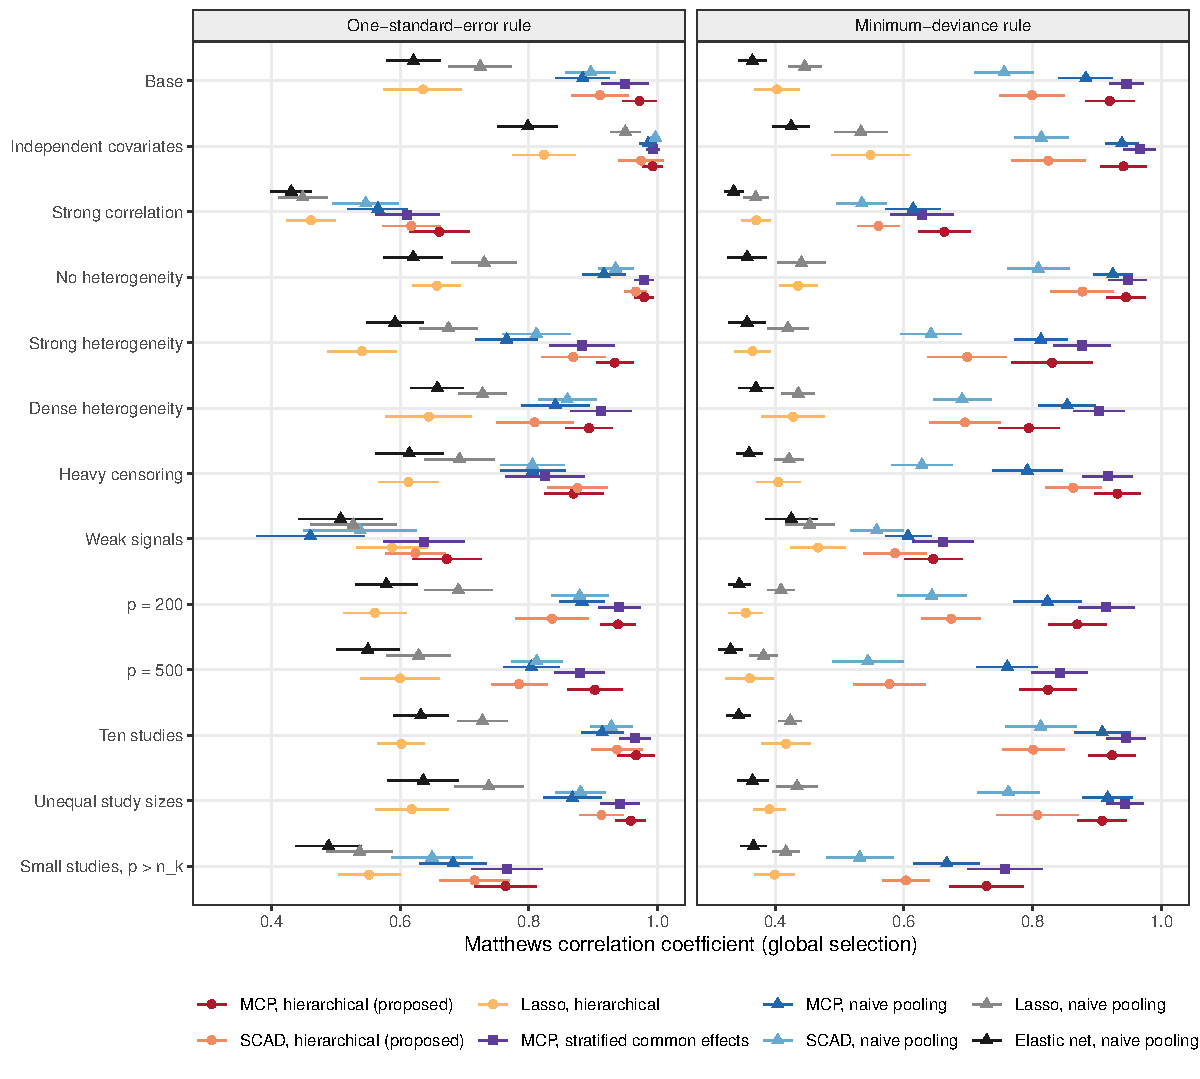
\includegraphics[width=0.9\textwidth]{figures/sim_mcc.pdf}
\caption{Matthews correlation coefficient of global selection in all scenarios,
under the one-standard-error rule (left) and the minimum rule (right). Bars:
$\pm1.96$ Monte Carlo standard errors.}
\label{fig:mcc}
\end{figure}

\begin{figure}[!htbp]
\centering
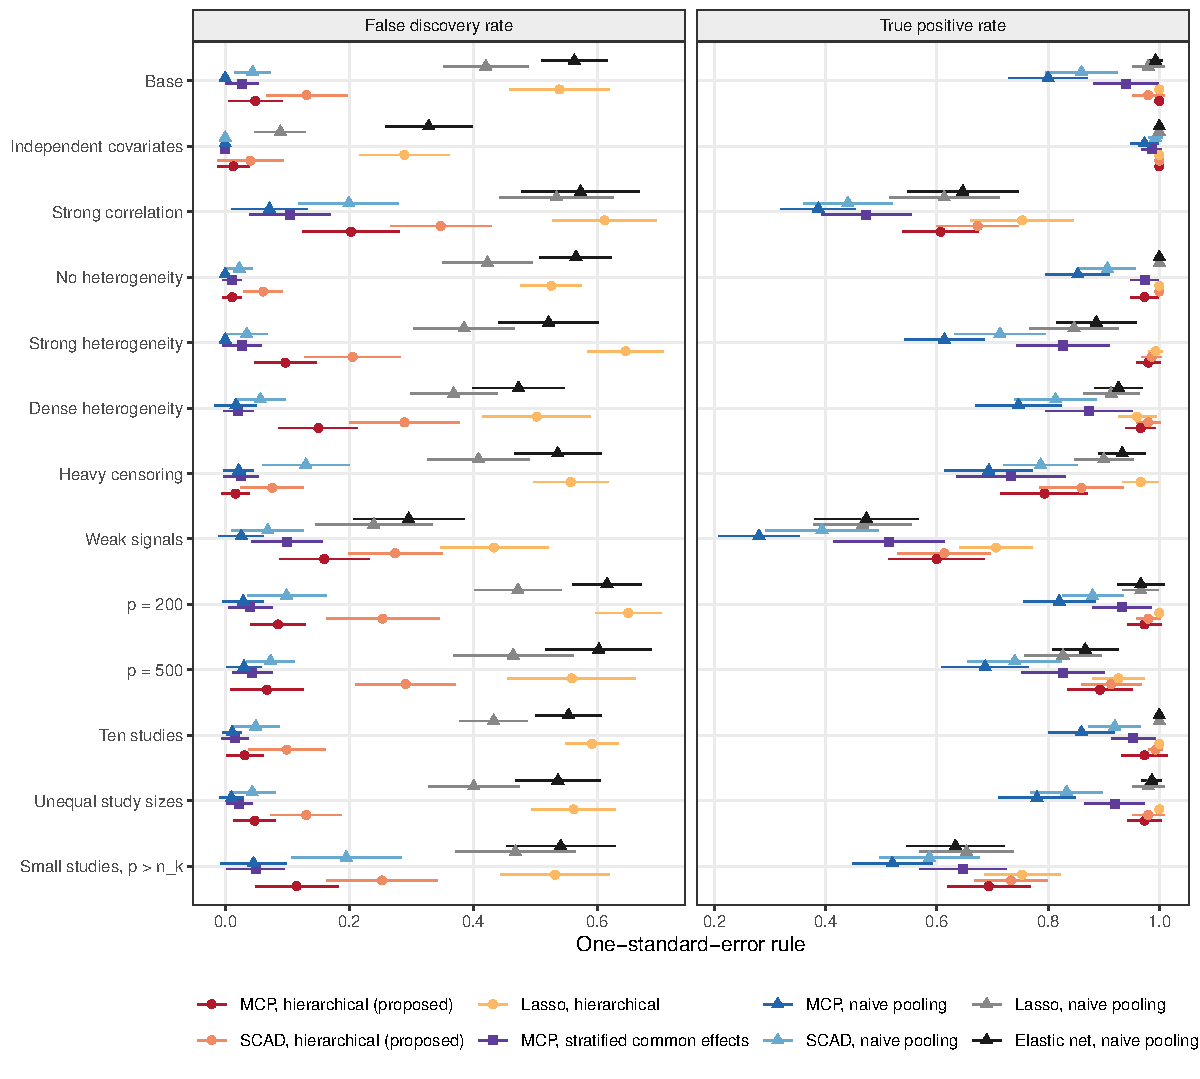
\includegraphics[width=0.9\textwidth]{figures/sim_fdr_tpr.pdf}
\caption{False discovery rate and true positive rate of global selection
(one-standard-error rule).}
\label{fig:fdrtpr}
\end{figure}

\begin{figure}[!htbp]
\centering
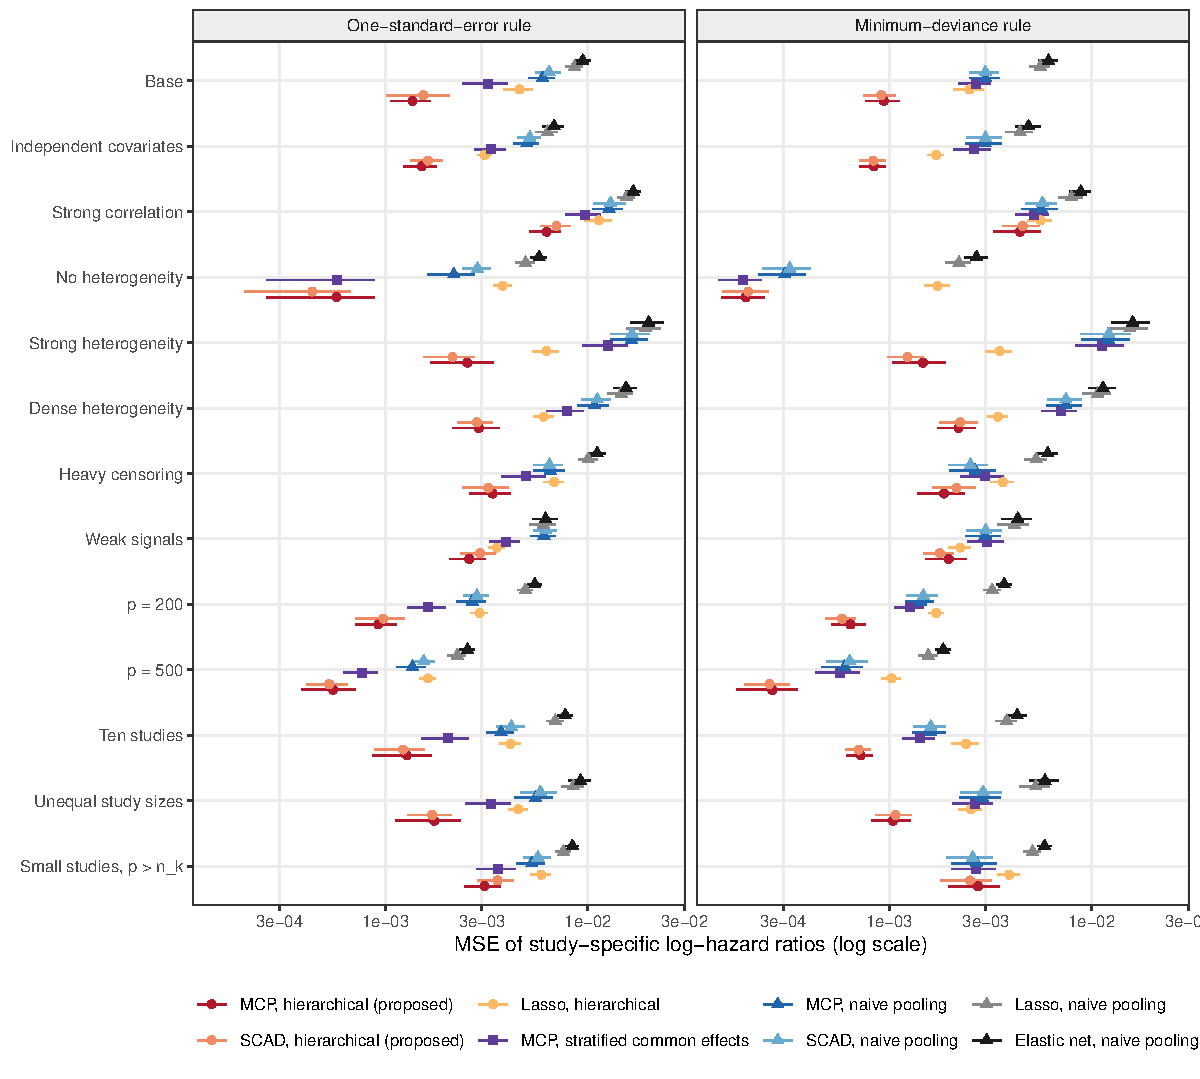
\includegraphics[width=0.9\textwidth]{figures/sim_mse_theta.pdf}
\caption{Mean squared error of the study-specific log-hazard ratios
$\hat\theta_{kj}$ (log scale).}
\label{fig:mse}
\end{figure}

\begin{figure}[!htbp]
\centering
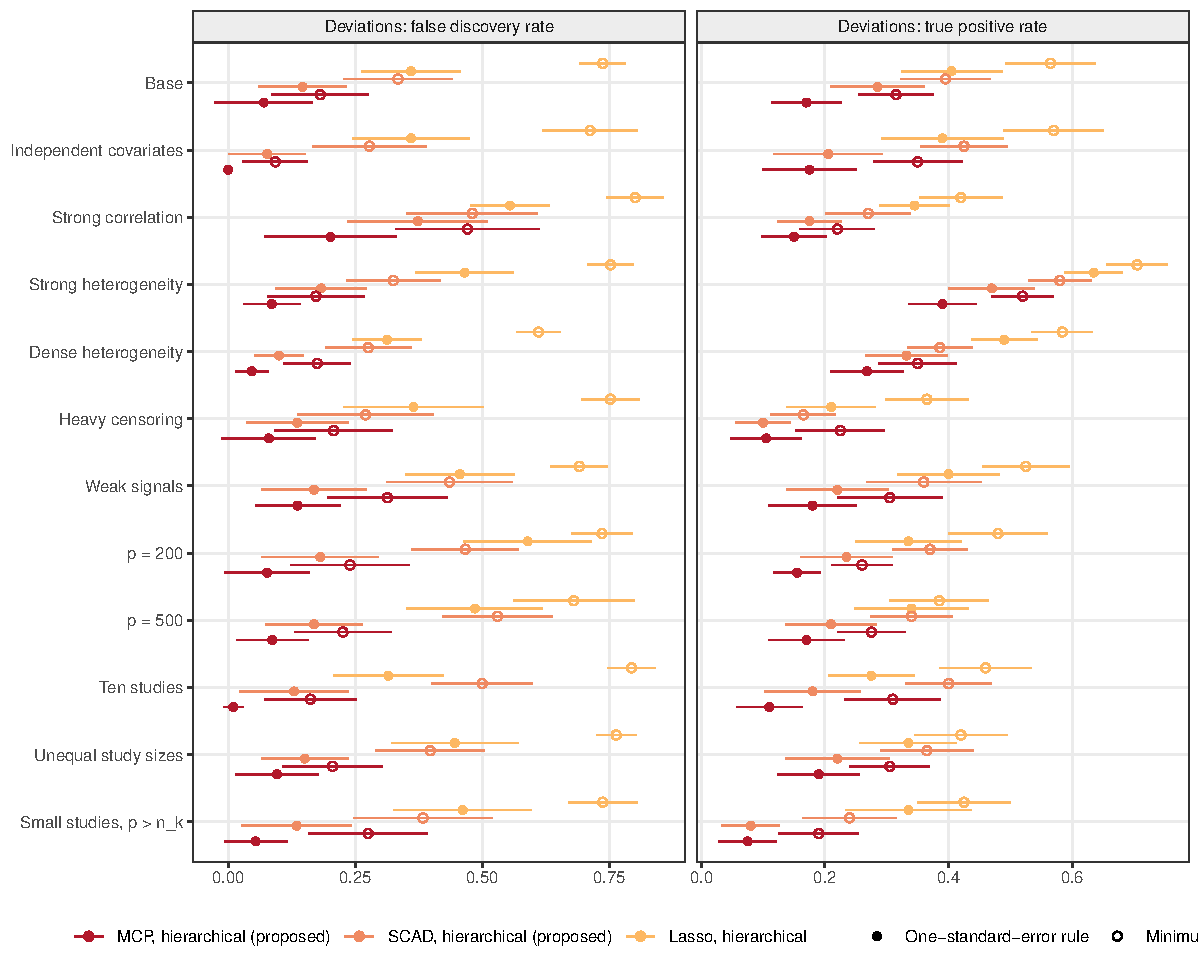
\includegraphics[width=0.9\textwidth]{figures/sim_deviations.pdf}
\caption{Recovery of the nonzero deviations by the three hierarchical estimators:
true positive rate and false discovery rate over the $Kp$ pairs $(k,j)$. Filled:
one-standard-error rule; open: minimum rule. The scenario without heterogeneity is
omitted because it has no true deviations.}
\label{fig:dev}
\end{figure}

\begin{table}[!htbp]
\centering\small
\caption{Hierarchical MCP: proportion of truly active covariates selected (TPR) and
empirical coverage of nominal 95\% post-selection Wald intervals for $\alpha_{0j}$
among selected active covariates, overall and for $|\alpha_{0j}|\ge0.5$.}
\label{tab:coverage}
\begin{adjustbox}{max width=\linewidth}\begin{tabular}{@{}lrrrrrr@{}}
\toprule
& \multicolumn{3}{c}{One-SE rule} & \multicolumn{3}{c}{Minimum rule} \\
\cmidrule(lr){2-4}\cmidrule(l){5-7}
Scenario & TPR & Cov. (all) & Cov. ($|\alpha_j|\ge 0.5$) & TPR & Cov. (all) & Cov. ($|\alpha_j|\ge 0.5$) \\
\midrule
Base & 1.000 & 0.813 & 0.730 & 1.000 & 0.820 & 0.760 \\
No heterogeneity & 0.973 & 0.884 & 0.900 & 1.000 & 0.940 & 0.940 \\
Strong heterogeneity & 0.980 & 0.694 & 0.667 & 1.000 & 0.800 & 0.730 \\
Heavy censoring & 0.793 & 0.689 & 0.621 & 0.947 & 0.782 & 0.717 \\
Weak signals & 0.600 & 0.644 & 0.560 & 0.740 & 0.739 & 0.720 \\
p = 500 & 0.893 & 0.687 & 0.646 & 0.987 & 0.750 & 0.687 \\
Small studies, $p>n_k$ & 0.693 & 0.596 & 0.562 & 0.793 & 0.605 & 0.582 \\
\bottomrule
\end{tabular}
\end{adjustbox}
\end{table}

% ══════════════════════════════════════════════════════════════════════════════
\section{Application: six ovarian cancer cohorts}
\label{sec:data}
% ══════════════════════════════════════════════════════════════════════════════

\subsection{Data and pre-processing}

We analysed overall survival in six cohorts of the Bioconductor package
\texttt{curatedOvarianData} \citep{Ganzfried2013}, which provides harmonised
gene-expression profiles and clinical annotation for published ovarian cancer
studies and has been used for cross-study validation of prognostic signatures
\citep{Waldron2014, Bernau2014}. We used the six cohorts analysed in the first
version of this paper: all participants with a recorded vital status and positive
follow-up were retained, giving $N=1{,}446$ patients and 735 deaths
(\cref{tab:cohorts}). The cohorts differ markedly in size (58 to 557 patients),
censoring (30\% to 59\%) and follow-up, and their Kaplan--Meier curves cross
(\cref{fig:km}), so a common baseline hazard is not tenable and stratification by
study is required.

Of the 12{,}249 genes measured in all six cohorts, we kept $p=500$ with an
outcome-blind filter: genes were ranked by their interquartile range within each
cohort, and the 500 with the best average rank were retained. The filter does not
use survival, so it does not bias the subsequent selection. With $p=500$, the
number of candidate genes exceeds the sample size of four of the six cohorts and
is 68\% of the total number of deaths. Each gene was standardised within cohort,
so hazard ratios are per within-cohort standard deviation. The first version of
this paper intersected the 2{,}000 most variable genes of each cohort and obtained
only $p=66$; the present filter gives a genuinely high-dimensional problem and a
gene set that does not depend on the platform-specific variability ranking of any
single cohort.

\begin{table}[!htbp]
\centering\small
\caption{Cohorts from \texttt{curatedOvarianData}. Median overall survival and
median follow-up (reverse Kaplan--Meier) are in years.}
\label{tab:cohorts}
\begin{adjustbox}{max width=\linewidth}\begin{tabular}{@{}llrrrrr@{}}
\toprule
Study & GEO/TCGA series & $n_k$ & Deaths & Censored (\%) & Median OS (yr) & Median follow-up (yr) \\
\midrule
A & TCGA & 557 & 290 & 48 & 3.70 & 4.30 \\
B & GSE32062.GPL6480 & 260 & 121 & 53 & 4.90 & 4.70 \\
C & GSE9891 & 276 & 113 & 59 & 3.90 & 3.00 \\
D & GSE26712 & 185 & 129 & 30 & 3.80 & 7.50 \\
E & GSE17260 & 110 & 46 & 58 & 4.40 & 3.90 \\
F & GSE30161 & 58 & 36 & 38 & 4.20 & 6.90 \\
\midrule
Total & & 1,446 & 735 & 49 & & \\
\bottomrule
\end{tabular}
\end{adjustbox}
\end{table}

\begin{figure}[!htbp]
\centering
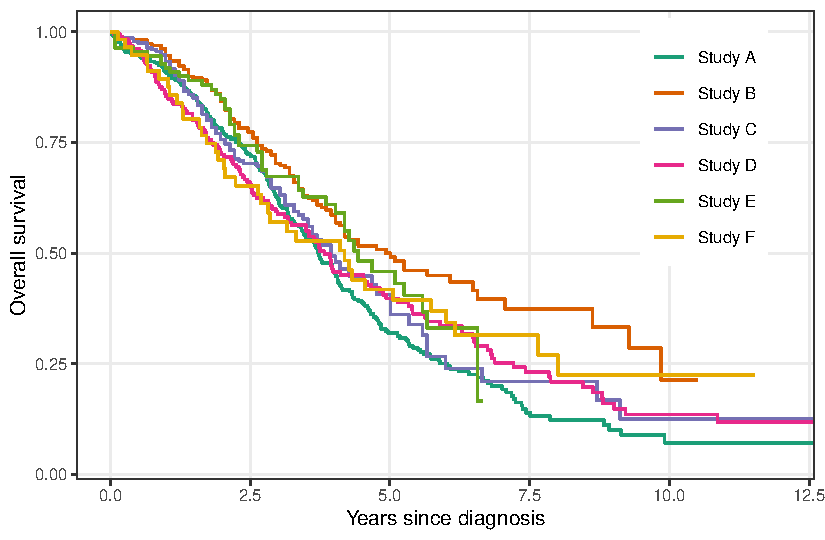
\includegraphics[width=0.7\linewidth]{figures/app_km.pdf}
\caption{Kaplan--Meier estimates of overall survival by cohort. The curves cross,
which argues against a common or proportional baseline hazard.}
\label{fig:km}
\end{figure}

\subsection{Analysis}

All eight methods of \cref{subsec:competitors} were applied with the same five
study- and event-stratified folds (seed 2026) and the settings of
\cref{subsec:tuning}. For the proposed MCP estimator we report the model chosen by
the minimum rule, whose purpose is to estimate study-specific effects, and we mark
which of its genes are also kept by the one-standard-error rule. For this model we
computed post-selection Wald intervals and $p$-values
(\cref{subsec:inference}), Holm-adjusted $p$-values across the selected genes,
and selection frequencies in 100 within-study bootstrap resamples refitted at the
selected $(\lambda_\alpha,\lambda_\varepsilon)$. Three sensitivity analyses were
carried out: (i) the number of folds, $V=10$ instead of 5; (ii) refitting the
selected genes in a Cox model with a shared gamma frailty for study instead of
stratification, and in a naively pooled Cox model; and (iii) cross-study validation,
in which each cohort in turn is held out, every method is tuned and fitted on the
other five, and Harrell's concordance index \citep{Harrell1996} of the global risk
score $\bx^\top\hat\balpha$ is computed in the held-out cohort \citep{Bernau2014}.

\subsection{Results}

\paragraph{Tuning and model size.}
\Cref{fig:cvsurface} shows the cross-validated deviance of the hierarchical MCP
model over the two-dimensional grid. The minimum is attained at $r=1$ and
$\lambda_\alpha=0.056$. The curve is flat near its minimum: the one standard
error of the deviance (16.2) spans all ratios $r\ge1$ over a range of
$\lambda_\alpha$, so the one-standard-error rule moves to the larger
$\lambda_\alpha=0.089$ with $r=2$, a two-gene model. The path is truncated
($d_{\max}=100$) well to the right of both choices, so the grid does not
constrain the selection.
The number of genes selected by each method is in \cref{tab:app_methods}. The
nonconvex methods select small models (hierarchical MCP 6 genes, stratified common-effect
MCP 4, MCP with naive pooling 8 under the minimum rule), whereas the lasso and the
elastic net with naive pooling select dozens of genes, in line with the false
discovery rates observed in \cref{sec:sim}.

\begin{figure}[!htbp]
\centering
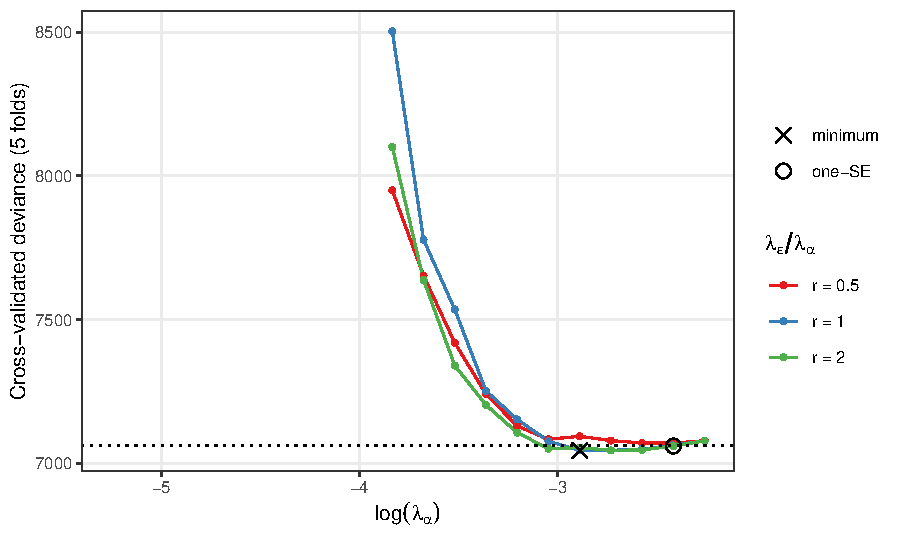
\includegraphics[width=0.75\linewidth]{figures/app_cv_surface.pdf}
\caption{Five-fold cross-validated deviance of the hierarchical MCP model as a
function of $\lambda_\alpha$ for the three ratios $r=\lambda_\varepsilon/\lambda_\alpha$.
Cross: minimum rule; circle: one-standard-error rule; dotted line: minimum plus
one standard error.}
\label{fig:cvsurface}
\end{figure}

\begin{table}[!htbp]
\centering\small
\caption{Number of genes (out of $p=500$) and of nonzero deviations selected by
each method under the minimum (min) and one-standard-error (1-SE) rules, and the
time for five-fold cross-validation.}
\label{tab:app_methods}
\begin{adjustbox}{max width=\linewidth}\begin{tabular}{@{}lrrrrr@{}}
\toprule
& \multicolumn{2}{c}{Genes selected} & \multicolumn{2}{c}{Deviations} & \\
\cmidrule(lr){2-3}\cmidrule(lr){4-5}
Method & min & 1-SE & min & 1-SE & CV time (s) \\
\midrule
MCP, hierarchical (proposed) & 6 & 2 & 1 & 0 & 18.5 \\
SCAD, hierarchical (proposed) & 8 & 7 & 0 & 0 & 10.4 \\
Lasso, hierarchical & 42 & 23 & 1 & 0 & 4.6 \\
MCP, stratified common effects & 4 & 2 & -- & -- & 4.4 \\
MCP, naive pooling & 8 & 4 & -- & -- & 12.7 \\
SCAD, naive pooling & 35 & 4 & -- & -- & 6.3 \\
Lasso, naive pooling & 56 & 11 & -- & -- & 23.8 \\
Elastic net, naive pooling & 59 & 13 & -- & -- & 24.8 \\
\bottomrule
\end{tabular}
\end{adjustbox}
\end{table}

\paragraph{Selected genes and their effects.}
\Cref{tab:app_genes} and \cref{fig:forest} report the six genes selected by the
hierarchical MCP model. Two genes are strongly supported: \textit{GMPR}
(HR 0.82, 95\% CI 0.76--0.89, Holm-adjusted $p=3.3\times10^{-6}$) and
\textit{CXCL9} (HR 0.84, 0.78--0.90, $p_{\rm Holm}=1.5\times10^{-5}$) are
associated with longer survival, and both are selected by all eight methods.
Higher expression of \textit{CRYAB} (HR 1.16, 1.08--1.25) and \textit{OSR2}
(HR 1.12, 1.04--1.22) is associated with shorter survival, and both remain
significant after Holm adjustment; \textit{GAS1} (HR 1.12, 1.03--1.22,
$p_{\rm Holm}=0.017$) is weaker. \textit{CXCL9} is a chemokine associated with
tumour-infiltrating T cells, and its favourable direction is consistent with the
known prognostic value of immune infiltration in high-grade serous ovarian
cancer; we do not attempt further biological interpretation.

The sixth gene, \textit{IGF2}, illustrates what the hierarchical model adds. Its
global effect is close to null (penalised HR 1.01; refitted HR 1.08, 95\% CI
0.99--1.17, $p=0.085$), but the model selects a deviation in Study~D (GSE26712),
where the hazard ratio is 1.33 (1.12--1.58). The association of \textit{IGF2} with
survival is thus concentrated in one cohort. A pooled or common-effect analysis
can only report the averaged hazard ratio (1.12--1.13 in \cref{tab:app_frailty}),
which is significant but misleading about how general the effect is; the first
version of this paper reported \textit{IGF2} as the strongest global signal for
exactly this reason. Note that the penalised $\exp(\hat\alpha_j)$ and the refitted
HR differ most for the weakest genes, where the MCP penalty is still in its
shrinking region.

\begin{table}[!htbp]
\centering\small
\caption{Genes selected by hierarchical MCP (minimum rule). $\exp(\hat\alpha_j)$:
penalised global hazard ratio per within-cohort SD. HR, 95\% CI and $p$: Wald
inference from the unpenalised stratified refit on the selected support
(\cref{subsec:inference}); $p_{\rm Holm}$: Holm-adjusted across the six genes.
Dev.: number of cohorts with a nonzero deviation. Boot.\ freq.: selection
frequency in 100 within-study bootstrap resamples. Methods: number of the eight
methods selecting the gene. $^\ast$Also selected under the one-standard-error rule.}
\label{tab:app_genes}
\begin{adjustbox}{max width=\linewidth}\begin{tabular}{@{}lrrrrrrcc@{}}
\toprule
Gene & $\exp(\hat\alpha_j)$ & HR & 95\% CI & $p$ & $p_{\rm Holm}$ & Dev. & Boot. freq. & Methods \\
\midrule
\textit{GMPR}$^{\ast}$ & 0.80 & 0.82 & (0.76, 0.89) & 5.5e-07 & 3.3e-06 & 0 & 0.49 & 8/8 \\
\textit{CXCL9} & 0.84 & 0.84 & (0.78, 0.90) & 2.9e-06 & 1.5e-05 & 0 & 0.65 & 8/8 \\
\textit{CRYAB} & 1.17 & 1.16 & (1.08, 1.25) & 0.0001 & 0.0004 & 0 & 0.26 & 8/8 \\
\textit{OSR2} & 1.10 & 1.12 & (1.04, 1.22) & 0.0032 & 0.0095 & 0 & 0.31 & 8/8 \\
\textit{GAS1} & 1.02 & 1.12 & (1.03, 1.22) & 0.0086 & 0.0172 & 0 & 0.19 & 7/8 \\
\textit{IGF2} & 1.01 & 1.08 & (0.99, 1.17) & 0.0853 & 0.0853 & 1 & 0.32 & 7/8 \\
\bottomrule
\end{tabular}
\end{adjustbox}
\end{table}

\begin{figure}[!htbp]
\centering
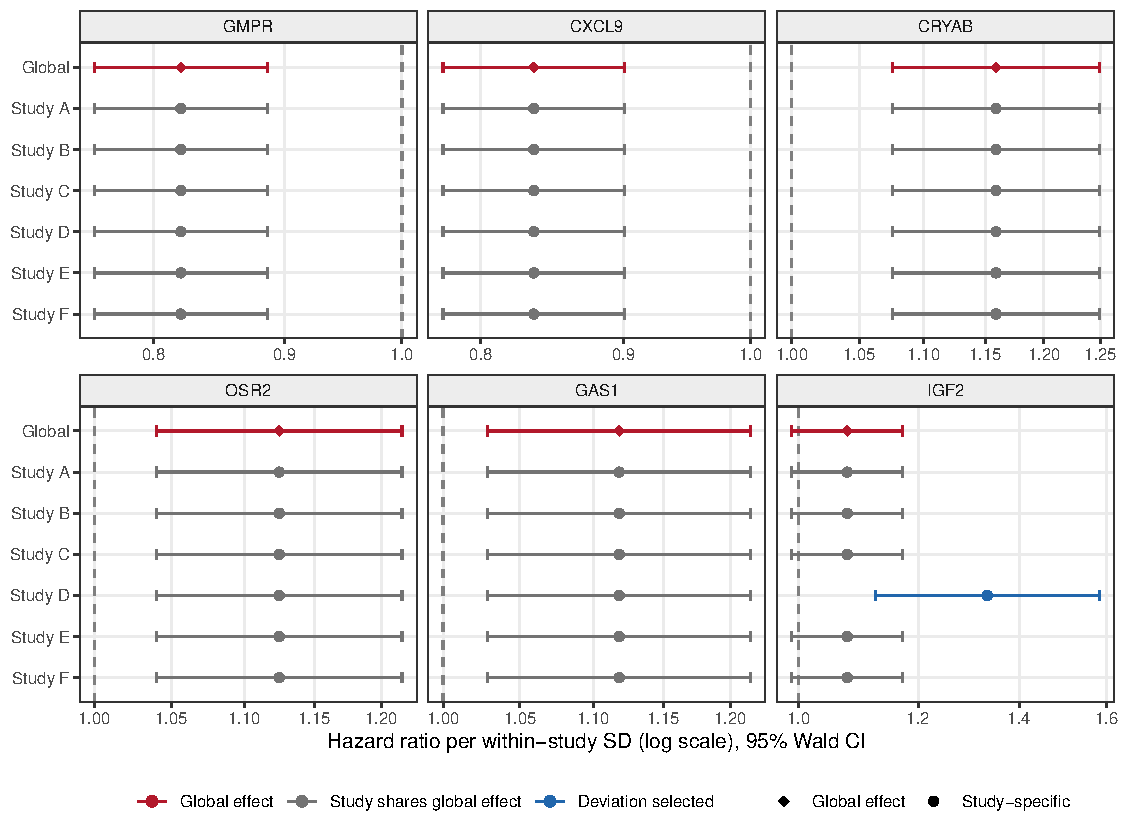
\includegraphics[width=0.85\textwidth]{figures/app_forest.pdf}
\caption{Global (red diamond) and study-specific (circles) hazard ratios with 95\%
Wald intervals for the six genes selected by hierarchical MCP. Blue: cohort with a
selected deviation; grey: cohort sharing the global effect, whose interval is
therefore that of the global effect.}
\label{fig:forest}
\end{figure}

\paragraph{Stability and sensitivity.}
Selection is only moderately stable
(\cref{fig:stability}). \textit{CXCL9} is selected in 65\% of bootstrap resamples
and \textit{GMPR} in 49\%; the other selected genes in 19\%--32\%. With $V=10$
folds, the minimum rule selects \textit{GMPR} and \textit{MFAP4}, and the
one-standard-error rule selects no gene; with $V=5$ the one-standard-error rule
also selects \textit{GMPR} and \textit{MFAP4}. \textit{GMPR} is therefore the one
gene selected under every tuning choice that selects any gene, whereas the
membership of the other genes depends on the tuning; the evidence for a
prognostic signal beyond \textit{GMPR} and \textit{CXCL9} is modest. The hazard ratios of the selected genes
are practically identical when study is handled by stratification, by a shared
gamma frailty, or ignored (\cref{tab:app_frailty}); the estimated frailty variance
is 0.018, so baseline differences between cohorts are small on the scale of these
gene effects and do not confound them. Stratification remains preferable because
it does not require proportional baselines, which \cref{fig:km} contradicts.

\begin{figure}[!htbp]
\centering
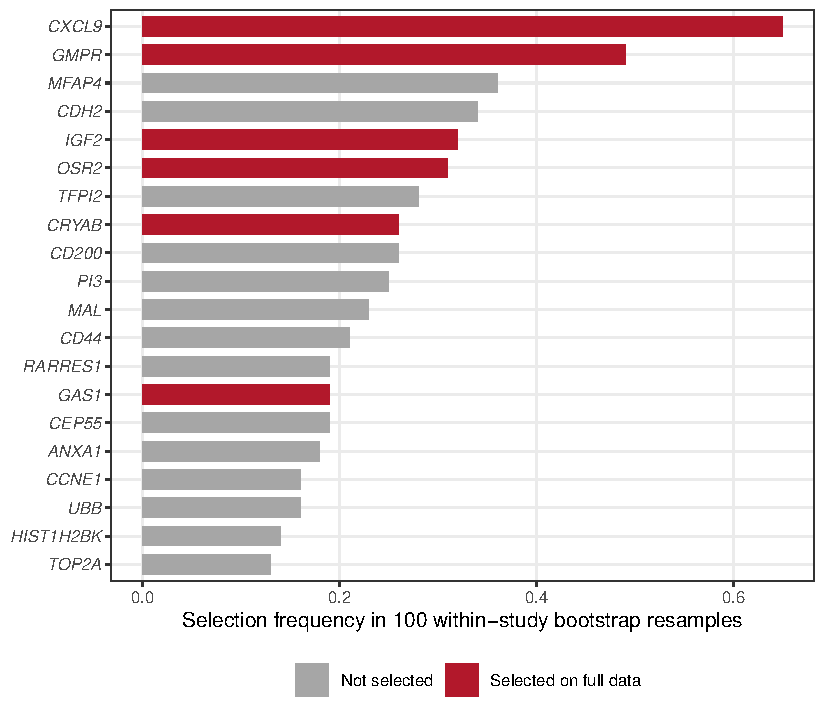
\includegraphics[width=0.7\linewidth]{figures/app_stability.pdf}
\caption{The 20 genes most often selected by hierarchical MCP in 100 within-study
bootstrap resamples at the tuning parameters chosen on the full data. Red: genes
selected on the full data.}
\label{fig:stability}
\end{figure}

\begin{table}[!htbp]
\centering\small
\caption{Hazard ratio (95\% CI) per within-cohort SD of the selected genes when
refitted jointly under three ways of handling the cohorts.}
\label{tab:app_frailty}
\begin{adjustbox}{max width=\linewidth}\begin{tabular}{@{}llll@{}}
\toprule
Gene & Stratified Cox & Shared gamma frailty & Naive pooling \\
\midrule
\textit{GMPR} & 0.82 (0.76, 0.89) & 0.83 (0.76, 0.89) & 0.83 (0.77, 0.90) \\
\textit{CXCL9} & 0.84 (0.78, 0.90) & 0.83 (0.77, 0.89) & 0.83 (0.77, 0.89) \\
\textit{CRYAB} & 1.16 (1.08, 1.25) & 1.16 (1.08, 1.25) & 1.16 (1.08, 1.25) \\
\textit{OSR2} & 1.13 (1.05, 1.22) & 1.13 (1.05, 1.23) & 1.14 (1.05, 1.23) \\
\textit{GAS1} & 1.11 (1.02, 1.21) & 1.11 (1.02, 1.20) & 1.11 (1.02, 1.20) \\
\textit{IGF2} & 1.12 (1.04, 1.21) & 1.13 (1.04, 1.22) & 1.13 (1.05, 1.22) \\
\bottomrule
\end{tabular}
\end{adjustbox}
\end{table}

\paragraph{Cross-study validation.}
\Cref{tab:app_loso} reports the concordance of the global risk
score in each held-out cohort. All values are modest (0.51--0.60), in line with
earlier cross-study evaluations of prognostic signatures in these data
\citep{Waldron2014, Bernau2014}. The dense models predict best: the elastic net and
the lasso with naive pooling reach a mean C of 0.60 with about 40 genes, against 0.56
for hierarchical MCP with about five genes (minimum rule). Under the
one-standard-error rule the sparse models often select no gene at all in the
training cohorts, and their C is close to 0.5. Hierarchical and common-effect MCP
give identical held-out predictions here, because the only deviation selected does
not alter the global effects used for prediction. The sparse models therefore give
up some predictive accuracy for a short, interpretable list of genes; when
prediction in new cohorts is the goal, a dense model is preferable.

\begin{table}[!htbp]
\centering\small
\caption{Leave-one-study-out validation: Harrell's C of the global risk score
$\bx^\top\hat\balpha$ in the held-out cohort, for each method tuned and fitted on
the other five cohorts, and the mean number of genes selected.}
\label{tab:app_loso}
\begin{adjustbox}{max width=\linewidth}\begin{tabular}{@{}lrrrrrr@{}}
\toprule
 & MCP-H & SCAD-H & MCP-S & MCP-P & LASSO-P & ENet-P \\
\midrule
\multicolumn{7}{@{}l}{\emph{Minimum rule}} \\
Study A held out & 0.549 & 0.565 & 0.549 & 0.595 & 0.598 & 0.597 \\
Study B held out & 0.542 & 0.549 & 0.542 & 0.562 & 0.583 & 0.581 \\
Study C held out & 0.605 & 0.610 & 0.605 & 0.610 & 0.656 & 0.656 \\
Study D held out & 0.587 & 0.637 & 0.587 & 0.611 & 0.607 & 0.611 \\
Study E held out & 0.579 & 0.590 & 0.579 & 0.592 & 0.600 & 0.598 \\
Study F held out & 0.505 & 0.511 & 0.505 & 0.562 & 0.572 & 0.580 \\
Mean C & 0.561 & 0.577 & 0.561 & 0.589 & 0.603 & 0.604 \\
Mean no.\ of genes & 4.7 & 9.2 & 4.7 & 9.8 & 38.3 & 42.7 \\
\midrule
\multicolumn{7}{@{}l}{\emph{One-standard-error rule}} \\
Study A held out & 0.500 & 0.500 & 0.500 & 0.551 & 0.575 & 0.577 \\
Study B held out & 0.500 & 0.565 & 0.500 & 0.558 & 0.564 & 0.564 \\
Study C held out & 0.603 & 0.612 & 0.603 & 0.615 & 0.606 & 0.607 \\
Study D held out & 0.500 & 0.500 & 0.500 & 0.500 & 0.638 & 0.640 \\
Study E held out & 0.500 & 0.567 & 0.500 & 0.547 & 0.546 & 0.549 \\
Study F held out & 0.465 & 0.528 & 0.465 & 0.465 & 0.555 & 0.561 \\
Mean C & 0.511 & 0.545 & 0.511 & 0.539 & 0.581 & 0.583 \\
Mean no.\ of genes & 0.5 & 2.3 & 0.5 & 1.8 & 9.5 & 10.0 \\
\bottomrule
\end{tabular}
\end{adjustbox}
\end{table}

\subsection{Conclusions from the application}
The analysis supports four conclusions. First, among 500 candidate
genes, \textit{GMPR} and \textit{CXCL9} are associated with longer overall survival
(hazard ratios 0.82 and 0.84 per SD, Holm-adjusted $p<10^{-4}$), selected by every
method and the most stable under resampling; \textit{CRYAB} and \textit{OSR2} are
associated with shorter survival but are less stable. Second, these effects are
common to all six cohorts: no deviation was selected for them, and the frailty and
stratified analyses agree. Third, the association of \textit{IGF2} with survival is
confined to one cohort (Study~D); this is the kind of finding that pooled or
common-effect analyses cannot make and that the hierarchical decomposition was
designed to reveal. Fourth, the prognostic signal in these expression data is weak
and diffuse: selection beyond the two leading genes depends on the tuning rule and
the number of folds, and dense models predict new cohorts somewhat better than any
sparse model. These conclusions are about genes; a clinical model would add stage,
grade and residual disease.

% ══════════════════════════════════════════════════════════════════════════════
\section{Discussion}
\label{sec:concl}
% ══════════════════════════════════════════════════════════════════════════════
We proposed a one-stage stratified Cox model for IPD meta-analysis in which each
study-specific log-hazard ratio is the sum of a global effect and a sparse,
fixed study-specific deviation, estimated by nonconvex penalised partial
likelihood under a hierarchy constraint and a sharing rule that identifies the
decomposition. Compared with the first version of this work, the objective
function is now stated explicitly, the zero-sum constraint has been replaced by an
identification rule compatible with sparse deviations, the two tuning parameters
are chosen by a fully specified two-dimensional cross-validation, and the method is
available as an R package with compiled code, tests, and scripts that regenerate
every result.

\paragraph{What the hierarchy adds.} The simulation separates three
ingredients. Stratification of the partial likelihood improves global selection in
every scenario; nonconvex penalties are necessary to control false discoveries,
whether or not the hierarchy is used; and the hierarchical deviations mainly improve
the estimation of study-specific effects, by a factor of 1.2 to 7.7 in squared error
when heterogeneity is present and at no cost when it is absent. With the
one-standard-error rule the hierarchical MCP estimator also gives the most accurate
global selection in most scenarios. The first version of this paper attributed the
lower false discovery rate to the decomposition; that comparison did not include a
stratified common-effect competitor and was based on an unstratified implementation,
and we no longer make that claim. In the application the hierarchy made one
substantive difference: it showed that the \textit{IGF2} association is confined to
one cohort.

\paragraph{Relation to frailty models.} Stratification and fixed deviations are an
alternative, not a replacement, to frailty and random-slope models
\citep{VaidaXu2000, RipattiPalmgren2000, Groll2017, Utazirubanda2021}. When the
number of studies is large and the question is the size of the between-study
variance, a random-effects formulation is natural. With the handful of studies
typical of IPD meta-analyses, many candidate covariates, and the question of
\emph{which} studies depart from a common effect, the fixed-deviation formulation
avoids a distributional assumption that cannot be checked and remains a penalised
partial likelihood. In our application the two formulations gave the same hazard
ratios for the selected genes.

\paragraph{Limitations.} First, the Wald intervals are conditional on the selected
model and under-cover in finite samples (\cref{tab:coverage}); they should be read
with the bootstrap selection frequencies, and selective-inference methods
\citep{Berk2013} for the stratified Cox model with a hierarchy constraint remain to
be developed. Second, the hierarchy constraint cannot represent a covariate that
acts only in a minority of studies other than through a small global effect with
large deviations; this is transparent in the output but may be undesirable when
such covariates are expected. Third, our simulation uses $R=25$ replicates per
scenario because of computational limits; Monte Carlo standard errors are
reported, and the differences we emphasise exceed them. Fourth, the theory covers
$p=O(N^c)$ with $c<1$; for $p\gg N$ a screening step \citep{Fan2008, Fan2010}
would be needed before penalisation. Fifth, the application uses gene expression
only; a clinical analysis would adjust for stage, grade and residual disease, which
are incompletely recorded across these cohorts.

\paragraph{Extensions.} Natural extensions are an information-criterion alternative
to cross-validation such as the extended BIC, group penalties for sets of
covariates such as pathways, time-varying deviations, and studies that measure
different subsets of covariates.


\section*{Code and data availability}
All code is openly available at \repo{} (release v1.0.0). The repository
contains the R package \texttt{hiermetacox}; the scripts
\path{simulation/01_run_simulation.R} and
\path{simulation/02_make_tables_figures.R}, which generate every simulation
table and figure in this paper; the scripts
\path{application/01_prepare_data.R}--\path{03_make_tables_figures.R},
which generate every table and figure of \cref{sec:data}; all per-replicate
simulation results; and a consistency check between code and manuscript. Tables
in this paper are \verb|\input| directly from files written by these scripts. The
ovarian cancer data are publicly available in the Bioconductor package
\texttt{curatedOvarianData} \citep{Ganzfried2013}. All computations used R 4.3.3
\citep{R2024}.

\bibliography{references}

\clearpage
\appendix
% ══════════════════════════════════════════════════════════════════════════════
\section{Proofs}
\label{app:proofs}
% ══════════════════════════════════════════════════════════════════════════════

\subsection{Set-up}
We work with the free parameter $\bvt\in\mathbb R^{(K+1)p_N}$ of \cref{sec:theory}.
Write $\ell_N(\bvt)=N^{-1}\sum_k\ell_k(\balpha+\beps_k)$, so that
$\mathcal Q_\lambda(\bvt)=-\ell_N(\bvt)+\mathcal P(\bvt)$ with $\mathcal P$ the penalty in
\eqref{eq:objective}, and denote by $\dot\ell_N$ and $\ddot\ell_N$ its gradient and
Hessian. The coordinate of $\bvt$ corresponding to $\alpha_j$ has design column
$\bx_{\cdot j}$; the coordinate corresponding to $\varepsilon_{kj}$ has column
$\bx_{\cdot j}\mathbf 1(\text{study}=k)$. The weights $\omega_k$ converge to positive
constants, so the deviation penalties $P(\omega_k|\cdot|;\lambda_\varepsilon,\gamma)$
satisfy Assumption~\ref{ass:penaltyshape} with $\lambda_\varepsilon$ replaced by
$\lambda_\varepsilon/\omega_k$, which is of the same order; we suppress $\omega_k$
below. For a vector $\mathbf v$ we write $\mathbf v_{\mathcal S}$ for its
subvector on $\mathcal S$.

\subsection{Auxiliary lemmas}

\begin{lemma}[Score]\label{lem:score_rate}
Under Assumptions~\ref{ass:censoring}--\ref{ass:bounded} and \ref{ass:dim},
$\|\dot\ell_N(\bvt_0)\|_\infty=O_P(\sqrt{\log p_N/N})$ and
$\|\dot\ell_{N,\mathcal S_0}(\bvt_0)\|_2=O_P(\sqrt{s_0/N})$.
\end{lemma}

\begin{proof}
In counting-process notation each coordinate of the score at the truth is
\[\dot\ell_{N,j}(\bvt_0)=N^{-1}\sum_k\int_0^{\tau_k}\phi_{kj}(t)\,dM_k(t),\]
with
$M_k$ the mean-zero martingale of study $k$ and $\phi_{kj}$ the predictable
covariate process of column $j$ centred at its risk-set average \emph{within
study $k$}; for a deviation coordinate of study $k'$, $\phi_{kj}\equiv0$ for
$k\neq k'$. By Assumption~\ref{ass:bounded}, $|\phi_{kj}|\le2M$, and by
Assumption~\ref{ass:baselinehazard} the compensator of $M_k$ is $O(n_k)$, so the
predictable variation of $\dot\ell_{N,j}(\bvt_0)$ is $O(N^{-1})$ uniformly in $j$.
Freedman's inequality for martingales with bounded jumps gives
$\Pr(|\dot\ell_{N,j}(\bvt_0)|>a)\le2\exp(-cNa^2)$ for small $a$ and a constant
$c$ not depending on $j$. A union bound over the $(K+1)p_N$ coordinates with
$a=M_0\sqrt{\log p_N/N}$ and $cM_0^2>1$ yields the first claim, because $K$ is
fixed. For the second, the covariance of $\dot\ell_{N,\mathcal S_0}(\bvt_0)$ has
trace $O(s_0/N)$ by the same bounds, and Markov's inequality applied to its
squared norm gives the rate.
\end{proof}

\begin{lemma}[Local expansion]\label{lem:quadratic_expansion}
Under Assumptions~\ref{ass:censoring}--\ref{ass:info}, uniformly over
$\mathcal N_N(C)=\{\bvt:\|\bvt-\bvt_0\|\le Cs_0^{1/2}N^{-1/2},\ \bvt_{\mathcal S_0^c}=\mathbf0\}$,
$\ell_N(\bvt)=\ell_N(\bvt_0)+(\bvt-\bvt_0)^\top\dot\ell_N(\bvt_0)
+\tfrac12(\bvt-\bvt_0)^\top\ddot\ell_N(\bvt_0)(\bvt-\bvt_0)+o_P(s_0/N)$, and with
probability tending to one
$c_1/2\le\lambda_{\min}(-\ddot\ell_{N,\mathcal S_0\mathcal S_0}(\bvt))\le
\lambda_{\max}(-\ddot\ell_{N,\mathcal S_0\mathcal S_0}(\bvt))\le2c_2$
on $\mathcal N_N(C)$.
\end{lemma}

\begin{proof}
Taylor's theorem gives the expansion with remainder
$\tfrac12(\bvt-\bvt_0)^\top\{\ddot\ell_N(\tilde\bvt)-\ddot\ell_N(\bvt_0)\}(\bvt-\bvt_0)$.
The uniform expansion in Assumption~\ref{ass:info} implies
$\sup_{\mathcal N_N(C)}\|\ddot\ell_{N,\mathcal S_0\mathcal S_0}(\bvt)-\ddot\ell_{N,\mathcal S_0\mathcal S_0}(\bvt_0)\|=o_P(1)$
and $\|{-\ddot\ell_{N,\mathcal S_0\mathcal S_0}(\bvt_0)}-N^{-1}\mathbf I_{N,\mathcal S_0}(\bvt_0)\|=o_P(1)$;
since $\|\bvt-\bvt_0\|^2=O(s_0/N)$ on $\mathcal N_N(C)$ the remainder is $o_P(s_0/N)$,
and the eigenvalue bounds follow from Assumption~\ref{ass:info} and Weyl's
inequality. Assumption~\ref{ass:structure}(ii) is used here: it ensures that the
columns indexed by $\mathcal S_0$ are not linearly dependent, so that
Assumption~\ref{ass:info} is not void.
\end{proof}

\begin{lemma}[Penalty]\label{lem:penalty_behavior}
Under Assumptions~\ref{ass:penaltyshape} and \ref{ass:penaltyrate}, for all large
$N$: $P'(|\alpha_{0j}|;\lambda_\alpha,\gamma)=0$ for $j\in\mathcal A_0$;
$P'(|\varepsilon_{0,kj}|;\lambda_\varepsilon,\gamma)=0$ for $j\in\mathcal A_0^{(k)}$;
and $P'(0+;\lambda,\gamma)=\lambda$. Moreover $P'(\cdot;\lambda,\gamma)$ vanishes
on a neighbourhood of radius $\gg d_N^{1/2}N^{-1/2}$ around each nonzero true
coefficient.
\end{lemma}

\begin{proof}
Immediate from the explicit derivatives of SCAD and MCP, which vanish on
$(\gamma\lambda,\infty)$, and from the minimum-signal conditions.
\end{proof}

\begin{lemma}[Oracle minimiser]\label{lem:oracle_maximizer}
Under Assumptions~\ref{ass:structure}--\ref{ass:dim}, with probability tending to
one the restriction of $\mathcal Q_\lambda$ to
$\{\bvt:\bvt_{\mathcal S_0^c}=\mathbf 0\}$ has a local minimiser $\hat\bvt^{o}$ with
$\|\hat\bvt^{o}-\bvt_0\|=O_P(s_0^{1/2}N^{-1/2})$, and $\hat\bvt^o\in\Hset$.
\end{lemma}

\begin{proof}
For $\|\mathbf u\|=Cs_0^{1/2}N^{-1/2}$ supported on $\mathcal S_0$ put
$D_N(\mathbf u)=\mathcal Q_\lambda(\bvt_0+\mathbf u)-\mathcal Q_\lambda(\bvt_0)$. By
\cref{lem:quadratic_expansion},
$D_N(\mathbf u)=-\mathbf u^\top\dot\ell_{N,\mathcal S_0}(\bvt_0)
-\tfrac12\mathbf u^\top\ddot\ell_{N,\mathcal S_0\mathcal S_0}(\bvt_0)\mathbf u
+\Delta_P(\mathbf u)+o_P(s_0/N)$. By Cauchy--Schwarz and \cref{lem:score_rate},
the linear term is $O_P(C s_0/N)$. The quadratic term is at least
$\tfrac14c_1C^2s_0/N$ with probability tending to one. By
\cref{lem:penalty_behavior} the penalty is locally constant around every nonzero
true coefficient, so $\Delta_P(\mathbf u)=0$ for large $N$. For $C$ large the
quadratic term dominates, so $D_N(\mathbf u)>0$ on the sphere and a local
minimiser exists in its interior. Every coordinate in $\mathcal S_0$ is bounded
away from zero by more than $Cs_0^{1/2}N^{-1/2}$ (Assumption~\ref{ass:penaltyrate}),
so $\hat\bvt^o$ has exactly the support $\mathcal S_0$; by
Assumption~\ref{ass:structure} this support satisfies \eqref{eq:sharing} and
\eqref{eq:hierarchy}, hence $\hat\bvt^o\in\Hset$.
\end{proof}

\subsection{Proof of \cref{thm:consistency}}
It suffices to show that $\hat\bvt^o$ of \cref{lem:oracle_maximizer} is, with
probability tending to one, a local minimiser of $\mathcal Q_\lambda$ over $\Hset$.
On $\mathcal S_0$ it is stationary by construction. For a coordinate $q\notin\mathcal S_0$
(an inactive global effect or an inactive deviation), $\hat\bvt^o$ is a local
minimiser in direction $q$ if $|\dot\ell_{N,q}(\hat\bvt^o)|<P'(0+)$, which equals
$\lambda_\alpha$ or $\lambda_\varepsilon$. A first-order expansion gives
$\dot\ell_{N,q}(\hat\bvt^o)=\dot\ell_{N,q}(\bvt_0)+\mathbf h_{N,q}^\top(\hat\bvt^o-\bvt_0)+o_P(N^{-1/2})$
uniformly in $q$, where $\mathbf h_{N,q}$ is the $q$th row of the Hessian at an
intermediate point, bounded in norm by Assumptions~\ref{ass:bounded} and
\ref{ass:info}. By \cref{lem:score_rate,lem:oracle_maximizer},
$\max_q|\dot\ell_{N,q}(\hat\bvt^o)|=O_P(\sqrt{\log p_N/N}+\sqrt{s_0/N})$, which is
$o_P(\min(\lambda_\alpha,\lambda_\varepsilon))$ by Assumptions~\ref{ass:penaltyrate}
and \ref{ass:dim}. Hence all Karush--Kuhn--Tucker inequalities hold strictly with
probability tending to one. Because the conditions are strict and the penalty is
flat near the nonzero coordinates, small perturbations in any direction that stay
in $\Hset$ do not decrease $\mathcal Q_\lambda$, so $\hat\bvt^o$ is a local minimiser
over $\Hset$ and $\hat\bvt=\hat\bvt^o$ has support $\mathcal S_0$. This gives both
claims. \hfill$\square$

\subsection{Proof of \cref{thm:oracle}}
On the event of \cref{thm:consistency}, $\hat\bvt=\hat\bvt^o$ and, by
\cref{lem:penalty_behavior}, the penalty has zero derivative at
$\hat\bvt_{\mathcal S_0}$, so $\dot\ell_{N,\mathcal S_0}(\hat\bvt)=\mathbf 0$. A Taylor
expansion around $\bvt_0$ gives
$\hat\bvt_{\mathcal S_0}-\bvt_{0,\mathcal S_0}=-\ddot\ell^{-1}_{N,\mathcal S_0\mathcal S_0}(\bvt^*)\dot\ell_{N,\mathcal S_0}(\bvt_0)$
with $\bvt^*\in\mathcal N_N(C)$, and \cref{lem:quadratic_expansion} yields
$\sqrt N(\hat\bvt_{\mathcal S_0}-\bvt_{0,\mathcal S_0})=\mathbf I^{-1}_{\mathcal S_0}(\bvt_0)\sqrt N\dot\ell_{N,\mathcal S_0}(\bvt_0)+o_P(1)$.
The active score is a sum over the $K$ independent studies of stochastic
integrals of bounded predictable processes against the study martingales, with
predictable variation converging to $\mathbf I_{\mathcal S_0}(\bvt_0)$; the martingale
central limit theorem \citep{AndersenGill1982} and Slutsky's theorem give the
result. The subvectors for $\balpha_{\mathcal A_0}$ and for each
$\beps_{k,\mathcal A_0^{(k)}}$ follow by projection. \hfill$\square$

\subsection{Proof of \cref{cor:coherence}}
By \cref{thm:consistency} and because $K$ is fixed,
$\hat{\mathcal A}^{(k)}=\mathcal A_0^{(k)}\subseteq\mathcal A_0=\hat{\mathcal A}$ for all $k$
simultaneously with probability tending to one, using
Assumption~\ref{ass:structure}(i). The second statement is
\cref{prop:convergence}(i). \hfill$\square$

\subsection{Proof of \cref{prop:convergence}}
(i) Steps (a)--(d) of the block update in \cref{subsec:algorithm} never produce
$\alpha_j=0$ with a nonzero deviation (step (b)), and step (d) leaves at least one
deviation equal to zero for every active covariate; step-halving takes a convex
combination of two points of $\Hset$ and is followed by setting to zero the
deviations of any covariate whose global effect has become zero, which does not
leave $\Hset$. (ii) The accept/halve rule accepts a new iterate only if
$\mathcal Q_\lambda$ has not increased, and otherwise returns the previous iterate.
(iii) $\mathcal Q_\lambda$ is bounded below because the penalties are nonnegative
and the negative log partial likelihood is bounded below by zero, so the
nonincreasing sequence converges. If the iterates converge to $\bar\bvt$, the
surrogate built at $\bar\bvt$ has the same gradient as $-\ell_N$ at $\bar\bvt$, and
$\bar\bvt$ is not moved by an exact coordinate minimisation of the penalised
surrogate; for every coordinate whose hierarchy constraint is inactive, exact
coordinate optimality of the surrogate at its expansion point is the
first-order condition of $\mathcal Q_\lambda$ in that coordinate. \hfill$\square$

% ══════════════════════════════════════════════════════════════════════════════
\section{Additional simulation results}
\label{app:sim}
\setcounter{table}{0}\renewcommand{\thetable}{A\arabic{table}}
% ══════════════════════════════════════════════════════════════════════════════
{\small\setlength{\tabcolsep}{4pt}
\begin{longtable}{@{}lrrrrrrrr@{}}
\caption{Monte Carlo means for all scenarios. MSE$(\theta)$ is multiplied by 100. Bold: best value within scenario and rule. Monte Carlo standard errors are in \texttt{simulation/results/sim\_summary.csv}.}\label{tab:sim_all}\\
\toprule
& \multicolumn{4}{c}{One-SE rule} & \multicolumn{4}{c}{Minimum rule} \\
\cmidrule(lr){2-5}\cmidrule(l){6-9}
Method & MCC & FDR & Exact & MSE$(\theta)$ & MCC & FDR & Exact & MSE$(\theta)$ \\
\midrule
\endfirsthead
\toprule Method & MCC & FDR & Exact & MSE$(\theta)$ & MCC & FDR & Exact & MSE$(\theta)$ \\ \midrule
\endhead
\bottomrule
\endlastfoot
\multicolumn{9}{@{}l}{\textbf{Base} ($R=25$)} \\
MCP-H & \textbf{0.972} & 0.049 & \textbf{0.76} & \textbf{0.136} & 0.920 & 0.137 & 0.44 & 0.094 \\
SCAD-H & 0.910 & 0.131 & 0.44 & 0.154 & 0.799 & 0.325 & 0.04 & \textbf{0.091} \\
LASSO-H & 0.635 & 0.539 & 0.04 & 0.460 & 0.403 & 0.780 & 0.00 & 0.250 \\
MCP-S & 0.949 & 0.027 & 0.68 & 0.320 & \textbf{0.946} & \textbf{0.082} & \textbf{0.56} & 0.268 \\
MCP-P & 0.884 & \textbf{0.000} & 0.36 & 0.598 & 0.883 & 0.189 & 0.28 & 0.299 \\
SCAD-P & 0.896 & 0.044 & 0.32 & 0.644 & 0.756 & 0.387 & 0.04 & 0.299 \\
LASSO-P & 0.724 & 0.421 & 0.04 & 0.859 & 0.446 & 0.749 & 0.00 & 0.558 \\
ENet-P & 0.621 & 0.563 & 0.00 & 0.945 & 0.365 & 0.812 & 0.00 & 0.613 \\
\midrule
\multicolumn{9}{@{}l}{\textbf{Independent covariates} ($R=25$)} \\
MCP-H & 0.992 & 0.013 & \textbf{0.96} & \textbf{0.151} & 0.941 & 0.100 & 0.60 & 0.084 \\
SCAD-H & 0.974 & 0.041 & 0.88 & 0.162 & 0.824 & 0.282 & 0.24 & \textbf{0.084} \\
LASSO-H & 0.823 & 0.289 & 0.12 & 0.310 & 0.548 & 0.636 & 0.04 & 0.171 \\
MCP-S & 0.993 & \textbf{0.000} & 0.92 & 0.334 & \textbf{0.966} & \textbf{0.059} & \textbf{0.72} & 0.263 \\
MCP-P & 0.985 & \textbf{0.000} & 0.84 & 0.498 & 0.939 & 0.108 & 0.44 & 0.299 \\
SCAD-P & \textbf{0.996} & \textbf{0.000} & \textbf{0.96} & 0.517 & 0.813 & 0.308 & 0.12 & 0.299 \\
LASSO-P & 0.950 & 0.089 & 0.52 & 0.632 & 0.533 & 0.663 & 0.00 & 0.444 \\
ENet-P & 0.798 & 0.328 & 0.12 & 0.681 & 0.425 & 0.765 & 0.00 & 0.488 \\
\midrule
\multicolumn{9}{@{}l}{\textbf{Strong correlation} ($R=25$)} \\
MCP-H & \textbf{0.661} & 0.203 & \textbf{0.04} & \textbf{0.626} & \textbf{0.663} & 0.429 & \textbf{0.00} & \textbf{0.443} \\
SCAD-H & 0.617 & 0.348 & 0.00 & 0.699 & 0.561 & 0.579 & \textbf{0.00} & 0.458 \\
LASSO-H & 0.462 & 0.612 & 0.00 & 1.134 & 0.371 & 0.803 & \textbf{0.00} & 0.560 \\
MCP-S & 0.611 & 0.104 & 0.00 & 0.964 & 0.628 & 0.392 & \textbf{0.00} & 0.517 \\
MCP-P & 0.566 & \textbf{0.071} & 0.00 & 1.273 & 0.614 & \textbf{0.357} & \textbf{0.00} & 0.565 \\
SCAD-P & 0.547 & 0.200 & 0.00 & 1.296 & 0.535 & 0.535 & \textbf{0.00} & 0.572 \\
LASSO-P & 0.449 & 0.534 & 0.00 & 1.552 & 0.370 & 0.802 & \textbf{0.00} & 0.796 \\
ENet-P & 0.431 & 0.573 & 0.00 & 1.678 & 0.336 & 0.828 & \textbf{0.00} & 0.885 \\
\midrule
\multicolumn{9}{@{}l}{\textbf{No heterogeneity} ($R=25$)} \\
MCP-H & \textbf{0.979} & 0.011 & \textbf{0.76} & 0.057 & 0.945 & 0.095 & \textbf{0.56} & 0.020 \\
SCAD-H & 0.966 & 0.061 & 0.60 & \textbf{0.044} & 0.877 & 0.203 & 0.28 & 0.020 \\
LASSO-H & 0.657 & 0.526 & 0.00 & 0.380 & 0.436 & 0.756 & 0.00 & 0.173 \\
MCP-S & \textbf{0.979} & 0.011 & \textbf{0.76} & 0.057 & \textbf{0.948} & \textbf{0.091} & \textbf{0.56} & \textbf{0.019} \\
MCP-P & 0.916 & \textbf{0.000} & 0.44 & 0.218 & 0.924 & 0.132 & 0.40 & 0.031 \\
SCAD-P & 0.935 & 0.023 & 0.44 & 0.285 & 0.809 & 0.311 & 0.12 & 0.032 \\
LASSO-P & 0.731 & 0.423 & 0.08 & 0.493 & 0.441 & 0.749 & 0.00 & 0.221 \\
ENet-P & 0.620 & 0.566 & 0.00 & 0.575 & 0.357 & 0.815 & 0.00 & 0.270 \\
\midrule
\multicolumn{9}{@{}l}{\textbf{Strong heterogeneity} ($R=25$)} \\
MCP-H & \textbf{0.933} & 0.097 & 0.44 & 0.254 & 0.830 & 0.269 & 0.32 & 0.147 \\
SCAD-H & 0.869 & 0.206 & 0.28 & \textbf{0.215} & 0.698 & 0.459 & 0.00 & \textbf{0.123} \\
LASSO-H & 0.541 & 0.646 & 0.00 & 0.625 & 0.365 & 0.810 & 0.00 & 0.352 \\
MCP-S & 0.882 & 0.027 & \textbf{0.48} & 1.257 & \textbf{0.876} & \textbf{0.147} & \textbf{0.36} & 1.132 \\
MCP-P & 0.766 & \textbf{0.000} & 0.04 & 1.640 & 0.813 & 0.259 & 0.08 & 1.213 \\
SCAD-P & 0.811 & 0.035 & 0.16 & 1.652 & 0.642 & 0.502 & 0.00 & 1.217 \\
LASSO-P & 0.675 & 0.385 & 0.00 & 1.928 & 0.420 & 0.755 & 0.00 & 1.547 \\
ENet-P & 0.592 & 0.522 & 0.00 & 1.998 & 0.356 & 0.809 & 0.00 & 1.595 \\
\midrule
\multicolumn{9}{@{}l}{\textbf{Dense heterogeneity} ($R=25$)} \\
MCP-H & 0.893 & 0.150 & 0.28 & 0.289 & 0.794 & 0.330 & 0.12 & \textbf{0.220} \\
SCAD-H & 0.809 & 0.289 & 0.20 & \textbf{0.283} & 0.695 & 0.463 & 0.08 & 0.225 \\
LASSO-H & 0.645 & 0.503 & 0.04 & 0.606 & 0.428 & 0.749 & 0.00 & 0.345 \\
MCP-S & \textbf{0.912} & 0.021 & \textbf{0.52} & 0.790 & \textbf{0.903} & \textbf{0.132} & \textbf{0.40} & 0.703 \\
MCP-P & 0.841 & \textbf{0.017} & 0.24 & 1.080 & 0.854 & 0.210 & 0.24 & 0.747 \\
SCAD-P & 0.860 & 0.057 & 0.20 & 1.115 & 0.690 & 0.464 & 0.00 & 0.747 \\
LASSO-P & 0.728 & 0.369 & 0.00 & 1.461 & 0.436 & 0.745 & 0.00 & 1.073 \\
ENet-P & 0.658 & 0.473 & 0.00 & 1.546 & 0.370 & 0.800 & 0.00 & 1.139 \\
\midrule
\multicolumn{9}{@{}l}{\textbf{Heavy censoring} ($R=25$)} \\
MCP-H & 0.869 & \textbf{0.017} & \textbf{0.40} & 0.339 & \textbf{0.932} & \textbf{0.068} & \textbf{0.56} & \textbf{0.187} \\
SCAD-H & \textbf{0.875} & 0.076 & \textbf{0.40} & \textbf{0.322} & 0.863 & 0.205 & 0.24 & 0.215 \\
LASSO-H & 0.613 & 0.558 & 0.00 & 0.682 & 0.405 & 0.779 & 0.00 & 0.365 \\
MCP-S & 0.824 & 0.026 & 0.32 & 0.497 & 0.916 & 0.070 & 0.52 & 0.296 \\
MCP-P & 0.806 & 0.022 & 0.12 & 0.652 & 0.792 & 0.321 & 0.16 & 0.266 \\
SCAD-P & 0.805 & 0.130 & 0.12 & 0.646 & 0.628 & 0.554 & 0.00 & 0.252 \\
LASSO-P & 0.692 & 0.409 & 0.04 & 1.004 & 0.422 & 0.770 & 0.00 & 0.533 \\
ENet-P & 0.614 & 0.536 & 0.00 & 1.111 & 0.360 & 0.816 & 0.00 & 0.607 \\
\midrule
\multicolumn{9}{@{}l}{\textbf{Weak signals} ($R=25$)} \\
MCP-H & \textbf{0.672} & 0.160 & 0.00 & \textbf{0.260} & 0.646 & 0.368 & \textbf{0.00} & 0.197 \\
SCAD-H & 0.624 & 0.274 & 0.00 & 0.294 & 0.586 & 0.521 & \textbf{0.00} & \textbf{0.178} \\
LASSO-H & 0.587 & 0.434 & 0.00 & 0.355 & 0.466 & 0.679 & \textbf{0.00} & 0.225 \\
MCP-S & 0.637 & 0.100 & \textbf{0.04} & 0.395 & \textbf{0.661} & \textbf{0.291} & \textbf{0.00} & 0.304 \\
MCP-P & 0.460 & \textbf{0.026} & 0.00 & 0.607 & 0.607 & 0.437 & \textbf{0.00} & 0.297 \\
SCAD-P & 0.538 & 0.069 & 0.00 & 0.619 & 0.558 & 0.541 & \textbf{0.00} & 0.300 \\
LASSO-P & 0.527 & 0.240 & 0.00 & 0.601 & 0.454 & 0.675 & \textbf{0.00} & 0.415 \\
ENet-P & 0.508 & 0.296 & 0.00 & 0.619 & 0.425 & 0.719 & \textbf{0.00} & 0.432 \\
\midrule
\multicolumn{9}{@{}l}{\textbf{p = 200} ($R=25$)} \\
MCP-H & 0.938 & 0.085 & 0.44 & \textbf{0.092} & 0.869 & 0.225 & 0.28 & 0.064 \\
SCAD-H & 0.836 & 0.254 & 0.20 & 0.098 & 0.674 & 0.517 & 0.00 & \textbf{0.058} \\
LASSO-H & 0.561 & 0.650 & 0.00 & 0.292 & 0.355 & 0.844 & 0.00 & 0.171 \\
MCP-S & \textbf{0.940} & 0.040 & \textbf{0.56} & 0.163 & \textbf{0.915} & \textbf{0.147} & \textbf{0.48} & 0.127 \\
MCP-P & 0.882 & \textbf{0.029} & 0.24 & 0.268 & 0.823 & 0.296 & 0.24 & 0.144 \\
SCAD-P & 0.879 & 0.099 & 0.32 & 0.283 & 0.644 & 0.551 & 0.04 & 0.148 \\
LASSO-P & 0.690 & 0.472 & 0.00 & 0.492 & 0.409 & 0.805 & 0.00 & 0.323 \\
ENet-P & 0.579 & 0.616 & 0.00 & 0.547 & 0.344 & 0.853 & 0.00 & 0.370 \\
\midrule
\multicolumn{9}{@{}l}{\textbf{p = 500} ($R=25$)} \\
MCP-H & \textbf{0.902} & 0.067 & \textbf{0.40} & 0.055 & 0.824 & 0.297 & 0.08 & 0.026 \\
SCAD-H & 0.785 & 0.291 & 0.04 & \textbf{0.053} & 0.578 & 0.639 & 0.00 & \textbf{0.026} \\
LASSO-H & 0.600 & 0.559 & 0.00 & 0.162 & 0.361 & 0.845 & 0.00 & 0.103 \\
MCP-S & 0.879 & 0.044 & 0.28 & 0.077 & \textbf{0.842} & \textbf{0.234} & \textbf{0.16} & 0.057 \\
MCP-P & 0.804 & \textbf{0.030} & 0.12 & 0.136 & 0.761 & 0.374 & 0.04 & 0.060 \\
SCAD-P & 0.812 & 0.073 & 0.04 & 0.155 & 0.544 & 0.646 & 0.00 & 0.064 \\
LASSO-P & 0.629 & 0.464 & 0.00 & 0.226 & 0.382 & 0.836 & 0.00 & 0.156 \\
ENet-P & 0.550 & 0.603 & 0.00 & 0.255 & 0.331 & 0.876 & 0.00 & 0.185 \\
\midrule
\multicolumn{9}{@{}l}{\textbf{Ten studies} ($R=25$)} \\
MCP-H & \textbf{0.966} & 0.031 & \textbf{0.76} & 0.127 & 0.923 & 0.131 & 0.44 & 0.072 \\
SCAD-H & 0.937 & 0.099 & 0.56 & \textbf{0.122} & 0.801 & 0.324 & 0.12 & \textbf{0.071} \\
LASSO-H & 0.602 & 0.592 & 0.00 & 0.416 & 0.417 & 0.768 & 0.00 & 0.240 \\
MCP-S & 0.965 & 0.016 & 0.72 & 0.204 & \textbf{0.944} & \textbf{0.096} & \textbf{0.60} & 0.142 \\
MCP-P & 0.914 & \textbf{0.011} & 0.40 & 0.372 & 0.908 & 0.154 & 0.48 & 0.160 \\
SCAD-P & 0.928 & 0.049 & 0.48 & 0.420 & 0.812 & 0.302 & 0.16 & 0.161 \\
LASSO-P & 0.728 & 0.433 & 0.00 & 0.690 & 0.424 & 0.769 & 0.00 & 0.381 \\
ENet-P & 0.632 & 0.554 & 0.00 & 0.774 & 0.344 & 0.827 & 0.00 & 0.429 \\
\midrule
\multicolumn{9}{@{}l}{\textbf{Unequal study sizes} ($R=25$)} \\
MCP-H & \textbf{0.958} & 0.048 & \textbf{0.60} & 0.174 & 0.908 & 0.156 & 0.36 & \textbf{0.105} \\
SCAD-H & 0.913 & 0.131 & 0.40 & \textbf{0.170} & 0.807 & 0.304 & 0.28 & 0.107 \\
LASSO-H & 0.618 & 0.562 & 0.00 & 0.453 & 0.391 & 0.793 & 0.00 & 0.253 \\
MCP-S & 0.941 & 0.023 & 0.52 & 0.331 & \textbf{0.944} & \textbf{0.098} & \textbf{0.56} & 0.265 \\
MCP-P & 0.868 & \textbf{0.010} & 0.32 & 0.551 & 0.917 & 0.142 & 0.52 & 0.290 \\
SCAD-P & 0.880 & 0.044 & 0.28 & 0.583 & 0.762 & 0.380 & 0.12 & 0.292 \\
LASSO-P & 0.738 & 0.401 & 0.04 & 0.847 & 0.434 & 0.756 & 0.00 & 0.531 \\
ENet-P & 0.636 & 0.537 & 0.00 & 0.920 & 0.365 & 0.811 & 0.00 & 0.589 \\
\midrule
\multicolumn{9}{@{}l}{\textbf{Small studies, $p>n_k$} ($R=25$)} \\
MCP-H & 0.764 & 0.115 & 0.08 & \textbf{0.309} & 0.728 & 0.292 & \textbf{0.04} & 0.275 \\
SCAD-H & 0.715 & 0.253 & 0.00 & 0.358 & 0.604 & 0.551 & 0.00 & \textbf{0.251} \\
LASSO-H & 0.552 & 0.532 & 0.00 & 0.589 & 0.399 & 0.790 & 0.00 & 0.393 \\
MCP-S & \textbf{0.766} & 0.049 & \textbf{0.12} & 0.361 & \textbf{0.757} & \textbf{0.194} & \textbf{0.04} & 0.270 \\
MCP-P & 0.682 & \textbf{0.046} & 0.00 & 0.529 & 0.666 & 0.368 & 0.00 & 0.270 \\
SCAD-P & 0.650 & 0.195 & 0.00 & 0.567 & 0.532 & 0.627 & 0.00 & 0.258 \\
LASSO-P & 0.537 & 0.468 & 0.00 & 0.757 & 0.417 & 0.777 & 0.00 & 0.511 \\
ENet-P & 0.489 & 0.541 & 0.00 & 0.839 & 0.366 & 0.821 & 0.00 & 0.586 \\
\end{longtable}
}

\end{document}

